\documentclass[letterpaper,11pt, oneside]{book}

% Idioma
\usepackage[spanish]{babel}
\usepackage{csquotes} % Facilidades avanzadas, complemento del idioma
\renewcommand{\spanishlisttablename}{Índice de tablas}
\renewcommand{\spanishtablename}{Tabla}

% Formato del documento
\usepackage[top=2cm, bottom=3.5cm, left=1cm, right=1cm]{geometry}
\setlength{\headheight}{1.8cm} % Espacio entre el header y el contenido de la página
% \usepackage[hidelinks]{hyperref}
\usepackage{hyperref}
\setlength{\parskip}{11pt} % Espacio entre párrafos

\usepackage{tocloft} % Habilitar la modificación de la tipografía de ToC, LoF, LoT
\newcommand{\divider}{ % Línea horizontal para los títulos de ToC, LoF, LoT
    \begin{center}
        \vspace*{-1.3cm}
        \rule{\textwidth}{1pt}
    \end{center}
}
\usepackage{float}

% Formato del Índice general (ToC)
\renewcommand{\cftbeforetoctitleskip}{5.4mm} % Espacio antes del título del ToC
\renewcommand{\cftaftertoctitleskip}{5mm}
\renewcommand{\cfttoctitlefont}{\huge\scshape}  % Título del ToC
\renewcommand{\cftchapfont}{\scshape}           % Títulos (capítulos en ToC)
\renewcommand{\cftchappagefont}{\scshape}       % Páginas (capítulos en ToC)
\addtocontents{toc}{\hfil\divider\protect\hfil\par}

% Formato del Índice de figuras (LoF)
\renewcommand{\cftbeforeloftitleskip}{5.4mm}    % Espacio antes del título del LoF
\renewcommand{\cftafterloftitleskip}{5mm}
\renewcommand{\cftloftitlefont}{\huge\scshape}  % Título del LoF
\addtocontents{lof}{\hfil\divider\protect\hfil\par}

% Formato del Índice de figuras (LoT)
\renewcommand{\cftbeforelottitleskip}{5.4mm}    % Espacio antes del título del LoT
\renewcommand{\cftafterlottitleskip}{5mm}
\renewcommand{\cftlottitlefont}{\huge\scshape}  % Título del LoT
\addtocontents{lot}{\hfil\divider\protect\hfil\par}

% Acrónimos
\usepackage[nohyperlinks]{acronym}

% Formato de los encabezados y pies de página
\usepackage{fancyhdr} % Personalizar los encabezados y pies de página
\fancyhf{} % Borrar la configuración por defecto
\lhead{
\includegraphics[height=15mm]{Images/LIESE-LogoName.pdf}} % Campo a la izquierda del encabezado (título del elemento en el nivel superior)
\rhead{\leftmark} % Campo a la derecha del encabezado (número de página)
\lfoot{\documento \\ \docID~(\version)~\fecha}
\rfoot{\thepage}
\renewcommand{\headrulewidth}{2pt} % Ancho de línea debajo del encabezado
\renewcommand{\footrulewidth}{2pt} % Ancho de línea arriba del pie de mágina

% Formato de los títulos
\usepackage{titlesec}
\titleformat{\chapter}[block]{\huge\scshape}{\raggedleft Capítulo~\thechapter \\ \rule{\textwidth}{1pt}}{1cm}{\huge}[\vspace{-0.8cm}\rule{\textwidth}{1pt}]
\titlespacing{\chapter}{0cm}{-2cm}{0cm}
\titleformat{\section}[block]{\Large\slshape}{\thesection}{0.8cm}{\Large}[\vspace{-0.8cm}\rule{\textwidth}{0.5pt}]
\titlespacing{\section}{0cm}{0cm}{0cm}
\titleformat{\subsection}[block]{\large\slshape}{\thesubsection}{0.8cm}{\large}
\titlespacing{\subsection}{0cm}{0cm}{0cm}
\titlespacing{\paragraph}{0cm}{0cm}{0cm}
\titlespacing{\subparagraph}{0.6cm}{0cm}{0.4cm}

\titleformat{\paragraph}
{\normalfont\normalsize\bfseries}{\theparagraph}{1em}{}
\titlespacing*{\paragraph}
{0pt}{3.25ex plus 1ex minus .2ex}{1.5ex plus .2ex}

\usepackage[width=0.75\textwidth]{caption} % Formato de las captions. Modificación del ancho de página del caption
\captionsetup[lstlisting]{labelformat=empty}
% Figuras
\usepackage{graphicx} % Manipulación de imágenes
\renewcommand{\cftfigfont}{Figura } % Nombre de las figuras en el LoF
\usepackage{wrapfig} % Colocar texto alrededor de las figuras
\usepackage{subcaption} % Manipulación de subfiguras

% Tablas
\usepackage{longtable} % Uso de tablas que continúan en la siguiente página
\usepackage{booktabs} % Uso de tablas más bonitas
\usepackage{multirow} % Uso de multirows en tablas
\usepackage{array} % Complemento para manejo de ambientes de tabulación
\renewcommand{\cfttabfont}{Tabla } % Nombre de las tablas en el LoT

% Entorno multicolumna
\usepackage{multicol}
\setlength{\columnseprule}{0.5pt}

% Matemáticas
\usepackage{amsmath} % Expresiones matemáticas
\usepackage{amssymb} % Colección de símbolos matemáticos
\usepackage{textcomp}
% Referencias
\usepackage[backend=biber, style=ieee, sorting=none]{biblatex}
\addbibresource{References.bib} % Archivo de referencias

% Otrosi

\usepackage{listings} % Ambiente para códigos de programación
\usepackage{xurl} % Permite los saltos de línea en cualquier caracter alfanúmerico en url grandes
\usepackage{gensymb}
\usepackage{tabularx}
\usepackage{footnote}
% \usepackage{times}
% \usepackage{svg}
% \svgsetup{inkscapelatex=false} % evita que use texto de LaTeX
\usepackage{upquote}

\graphicspath{{./Images/}{./Images/Parte1}{./Images/Parte2}}

\usepackage[dvipsnames, svgnames,table, x11names]{xcolor}

\definecolor{githubgray}{rgb}{0.95,0.95,0.95} % Fondo de los bloques de código de GitHub

\definecolor{githubpurple}{rgb}{0.4,0.1,0.4} % Color para los comentarios de MATLAB

\lstdefinestyle{mystyle}{
    language=bash,
	basicstyle=\small\ttfamily,
	backgroundcolor=\color{githubgray},
	keywordstyle=\color{blue},
	commentstyle=\color{violet},
	stringstyle=\color{red},
	% numbers=left,
	% numberstyle=\tiny,
	% numbersep=5pt,
	breaklines=true,
	showstringspaces=false,
    breakatwhitespace=false,
    keepspaces=true,
    columns=fullflexible,
    upquote=true,
    showstringspaces=false,
    % frame=single,
	tabsize=2,
	%	frame=single,
	framexleftmargin=3mm,
	framexrightmargin=3mm,
	framextopmargin=3mm, % Margen superior
	framexbottommargin=3mm, % Margen inferior
	xleftmargin=10mm,
	xrightmargin=10mm,
	framesep=5pt,
	aboveskip=10pt,
	belowskip=10pt,
    caption= ,
    captionpos=b,
	% xleftmargin=.1\textwidth, xrightmargin=.1\textwidth,
	escapeinside={(*@}{@*)}, % Si quieres añadir comentarios LaTeX dentro del código MATLAB
    title={},
    literate={@}{{@}}1{.}{{.}}1{"}{{"}}1
}

\lstset{style=mystyle, caption={}, label={}}
\lstdefinelanguage{bash}{
  keywords={sudo, nano, ls, cd, mkdir, rm, mv, cp, echo, cat, chmod, chown, apt, apt-get, yum, systemctl, git, make, export, tar, alias, ssh},
  sensitive=true,
  morecomment=[l]{\#},
  morestring=[b]",
  morestring=[b]',
}

% \renewcommand{\lstlistingname}{C\'odigo}% Listing -> Algorithm
% \renewcommand{\lstlistlistingname}{Lista de \lstlistingname s}% List of Listings -> List of Algorithms


% \definecolor{vgreen}{RGB}{104,180,104}
% \definecolor{vblue}{RGB}{49,49,255}
% \definecolor{vorange}{RGB}{255,143,102}

% \lstdefinestyle{verilog-style}
% {
%     basicstyle=\footnotesize\ttfamily,
% 	backgroundcolor=\color{githubgray},
% 	numbers=left,
% 	numberstyle=\tiny,
% 	numbersep=5pt,
% 	breaklines=true,
% 	showstringspaces=false,
% 	tabsize=2,
% 	%	frame=single,
% 	framexleftmargin=5mm,
% 	framexrightmargin=5mm,
% 	framextopmargin=2mm, % Margen superior
% 	framexbottommargin=2mm, % Margen inferior
% 	xleftmargin=20mm,
% 	xrightmargin=20mm,
% 	framesep=5pt,
% 	captionpos=b,
% 	aboveskip=10pt,
% 	belowskip=10pt,
% 	caption=\lstname,
%     language=Verilog,
%     keywordstyle=\color{vblue},
%     identifierstyle=\color{black},
%     commentstyle=\color{vgreen},
%     moredelim=*[s][\colorIndex]{[}{]},
%     literate=*{:}{:}1
% }

 


\makeatletter
\newcommand*\@lbracket{[}
\newcommand*\@rbracket{]}
\newcommand*\@colon{:}
\newcommand*\colorIndex{%
    \edef\@temp{\the\lst@token}%
    \ifx\@temp\@lbracket \color{black}%
    \else\ifx\@temp\@rbracket \color{black}%
    \else\ifx\@temp\@colon \color{black}%
    \else \color{vorange}%
    \fi\fi\fi
}
\makeatother

\usepackage{trace}
\usepackage{wrapfig}

% \let\oldref\ref
% \renewcommand{\ref}[1]{\textcolor{red}{\oldref{#1}}}
\newcommand{\n}{\~n}
\newcommand{\ais}{FPGA AI Suite }

% Para \ref
\let\oldref\ref
\renewcommand{\ref}[1]{\textcolor{blue}{\oldref{#1}}}

% Para \url
% \let\oldurl\url
% \renewcommand{\url}[1]{{\oldurl{#1}}}
\newcommand{\curl}[1]{\textcolor{Turquoise4}{\url{#1}}}
\newcommand{\comm}[1]{\textcolor{blue}{\texttt{{#1}}}}
\newcommand{\cbut}[1]{\textcolor{DarkOrchid1}{\texttt{{#1}}}}
\newcommand{\cred}[1]{\textcolor{red}{\texttt{{#1}}}}

% Para \hyperref (opcional)
\let\oldhyperref\hyperref
\renewcommand{\hyperref}[2][]{\oldhyperref[#1]{\textcolor{blue}{#2}}}


\newcommand{\cref}[1]{\hyperref[#1]{\textcolor{magenta}{figura \ref*{#1}}}}
\newcommand{\ctref}[1]{\hyperref[#1]{\textcolor{magenta}{tabla \ref*{#1}}}}


% DEFINICIÓN DE VARIABLES
% Al modificar el contenido de las variables se actualizarán los datos correspondientes en el documento.
% * * * * * * * * * * * * * * * * * * * * * * * * * * * * * * * * * * * * * * * * * * * *

\def\unam      {Universidad Nacional Autónoma de México}
\def\fing      {Facultad de Ingeniería}
\def\liese     {Laboratorio de Instrumentación Electrónica de Sistemas Espaciales}
\def\proyecto  {Artificial Neuronal Network}
\def\serie     {Manual de capacitaci\'on}
\def\documento {Uso de la tarjeta Agilex 7 FPGA I-Series Transceiver-SoC Development Kit}
\def\docID     {ANN-MAN-FPGA}
\def\version   {v0.0} % Modificar la versión una vez que se aprueben las modificaciones
\def\fecha     {3 de marzo de 2025} % Modificar la fecha una vez que se aprueben las modificaciones
\def\agilex    {Agilex 7 FPGA I-Series Transceiver-SoC Development Kit}
\def\bts       {Board Test System }
\def\quartus   {Quartus Prime Pro Edition }


\begin{document}

%---------------------------------

 % \frotnmatter indica la primera parte del documento, enumerando las páginas con números romanos (I, II, III, ...), sin considerar una numeración para los capítulos, aunque estos sí aparezcan en el tableofcontents
%    \frontmatter
%
%    % El archivo 'portada.tex' contiene el formato de la portada del documento, la cual no debe modificarse. El título, número de documento y la versión se actualiza automáticamente a partir de las variables del archivo 'main.tex'
%        
%        \begin{titlepage}
    \setlength{\parindent}{0in}
    \vspace*{3cm}
    {\Huge \bfseries \proyecto}
    
    \vspace*{3cm}
    {\huge \scshape \serie}

    \vspace*{5mm}
    \hrule
    \vspace*{5mm}
    {\LARGE \scshape \documento}
    
    \vspace*{4cm}
    \hrule
    \vspace*{5mm}
    {\large \docID~(\version)~\fecha}
    \vfill
    \hfill
    
\includegraphics[width=8cm]{Images/LIESE-LogoName.pdf}
\end{titlepage}
%
%        \pagestyle{fancy} % A partir de aquí se aplica el estilo fancy definido en el archivo config.tex
%
%        % El archivo 'Historial de versiones.tex' se debe de modificar después de que se aprueben las modificaciones del documento.
%         \chapter{Historial de versiones}
La siguiente tabla muestra el historial de las versiones de este documento.

\begin{table}[h!]
    \centering
    \begin{tabular}{p{1.5cm} p{2cm} p{5cm} p{9cm}}
        Versión & Fecha & Autor & Resumen de los cambios \\ \hline
        v0.0 & 3/03/2025 & F\'elix Garc\'ia & Creación del documento. \\
        v1.1 & 5/03/2025 & F\'elix Garc\'ia & Creación del cap\'itulo 1 y 2. \\
        v1.2 & 11/03/2025 & F\'elix Garc\'ia & Cambio del formato y estructura. \\
        v1.3 & 12/03/2025 & F\'elix Garc\'ia & Creaci\'on del cap\'itulo 3. \\
        v1.4 & 31/03/2025 & F\'elix Garc\'ia & Creaci\'on del cap\'itulo 4. \\
        v1.5 & 28/05/2025 & F\'elix Garc\'ia & Correcci\'on de errores y terminaci\'on del cap\'itulo 4. \\
        v1.6 & 11/06/2025 & F\'elix Garc\'ia & Anexo de contenidos al cap\'itulo 1. \\
        v1.7 & 16/06/2025 & F\'elix Garc\'ia & Anexo de contenidos al cap\'itulo 2. \\
    \end{tabular}
\end{table}
%    
%        \hypersetup{linkcolor=black, citecolor=black, urlcolor=black}
%    
%         \clearpage\tableofcontents % Índice general
%         \clearpage\listoffigures % Índice de figuras
%         \clearpage\listoftables % Índice de tablas
%
%        % El archivo 'Acronimos.tex' enlista los acrónimos utilizados en el documento. Se debe de actualizar conforme se vayan añadiendo nuevos acrónimos.
%         \chapter{Lista de acrónimos}

\begin{acronym}[UNAM]  % Entre corchetes se coloca el acrónimo más grande para que se genere el espaciado correcto.
    \acro{FPGA}{Field Programmable Gate Array}
    \acro{LIESE}{Laboratorio de Instrumentación Electrónica de Sistemas Espaciales}
    \acro{UNAM}{Universidad Nacional Autónoma de México}
    \acro{CLB}{Configurable Logic Block}
    \acro{LAB}{Logic Array Block}
    \acro{SoC}{System on Chip}
    \acro{BTS}{Board Test System}
    \acro{GUI}{Graphical User Interface}
    \acro{HPS}{Hard Processor System}
    \acro{SDM}{Secure Device Manager}
    \acro{FHT}{High speed transceiver block}
    \acro{FGT}{General purpouse transceiver block}
    \acro{QSPI}{Quad Serial Peripheral Interface}
    \acro{OOBE}{Out of Box Experience}
    \acro{JTAG}{Joint Test Action Group}
    \acro{FMC/FMC+}{FPGA Mezzanine Card/FPGA Mezzanine Card Plus}
    \acro{MCIO}{Multi-Connector I/O}
    \acro{QSFPDD}{Quad Small Form-Factor Pluggable Double Density}
    \acro{ECC}{Error Correcting Code}
    \acro{M2M}{Memory to Memory}
    \acro{S2M}{Streaming to Memory}
    
\end{acronym}
%
%        % \mainmatter indica el contenido principal del documento, reiniciando la numeración de páginas y usando números arábigos (1, 2, 3, ...).
%    \mainmatter

%     \chapter{Acerca de la tarjeta Agilex 7 I-Series}

\section{Inicio}

    La tarjeta Agilex 7 FPGA I-Series Transceiver-SoC Development Kit es un entorno de dise\n o completo que incluye el software y el hardware necesarios para realizar diseños para trabajar con las FPGAs de la familia Agilex 7 I-Series, las cuales son FPGAs de alto rendimiento orientadas a c\'omputo, redes y comunicaciones.
    
    En este cap\'itulo se da una introducci\'on del kit de desarrollo, el cual tiene como objetivo facilitar la evaluaci\'on y desarrollo de soluciones con alto rendimiento de transceptores\footnote{Un transceptor es un bloque de hardware que facilita la comunicaci\'on serial de alta velocidad. En FPGAs son esenciales para la comunicaci\'on de dato de alta velocidad, serializaci\'on y deserializaci\'on de datos, adaptaci\'on de protocolos, manejo de errores y otras tareas en aplicaciones que exigen un alto desempe\n o, baja latencia y flexibilidad. }.

    \begin{figure}[H]
        \centering
        \includegraphics[width=0.8\linewidth]{agilex1.png}
        \caption{Vista superior de la tarjeta Agilex 7 FPGA I-Series Transceiver-SoC Development Kit.}
        % \label{fig:enter-label}
   \end{figure}

   \subsection{Diagrama de bloques}

        En la \cref{fig:block} se presenta el diagrama de bloques de la tarjeta de desarrollo, el cual muestra c\'omo se interconectan los componentes principales del kit, incluyendo los tranceptores FGT\footnote{General purpouse transceiver block} y FHT\footnote{High speed transceiver block}, interfaces de memoria DDR4, conectores FMC+\footnote{FPGA Mezzanine Card Plus}, MCIO\footnote{Multi-Connector I/O} y QSFPDD\footnote{Quad Small Form-Factor Pluggable Double Density}, entre otros.
   
   \begin{figure}[H]
       \centering
       \includegraphics[width=\linewidth]{Images//Parte1/blocks.png}
       \caption{Diagrama de bloques de la tarjeta Agilex 7 FPGA I-Series Transceiver-SoC Development Kit.}
       \label{fig:block}
   \end{figure}

\subsection{Elementos de la tarjeta de desarrollo.}

    \begin{figure}[H]
        \centering
        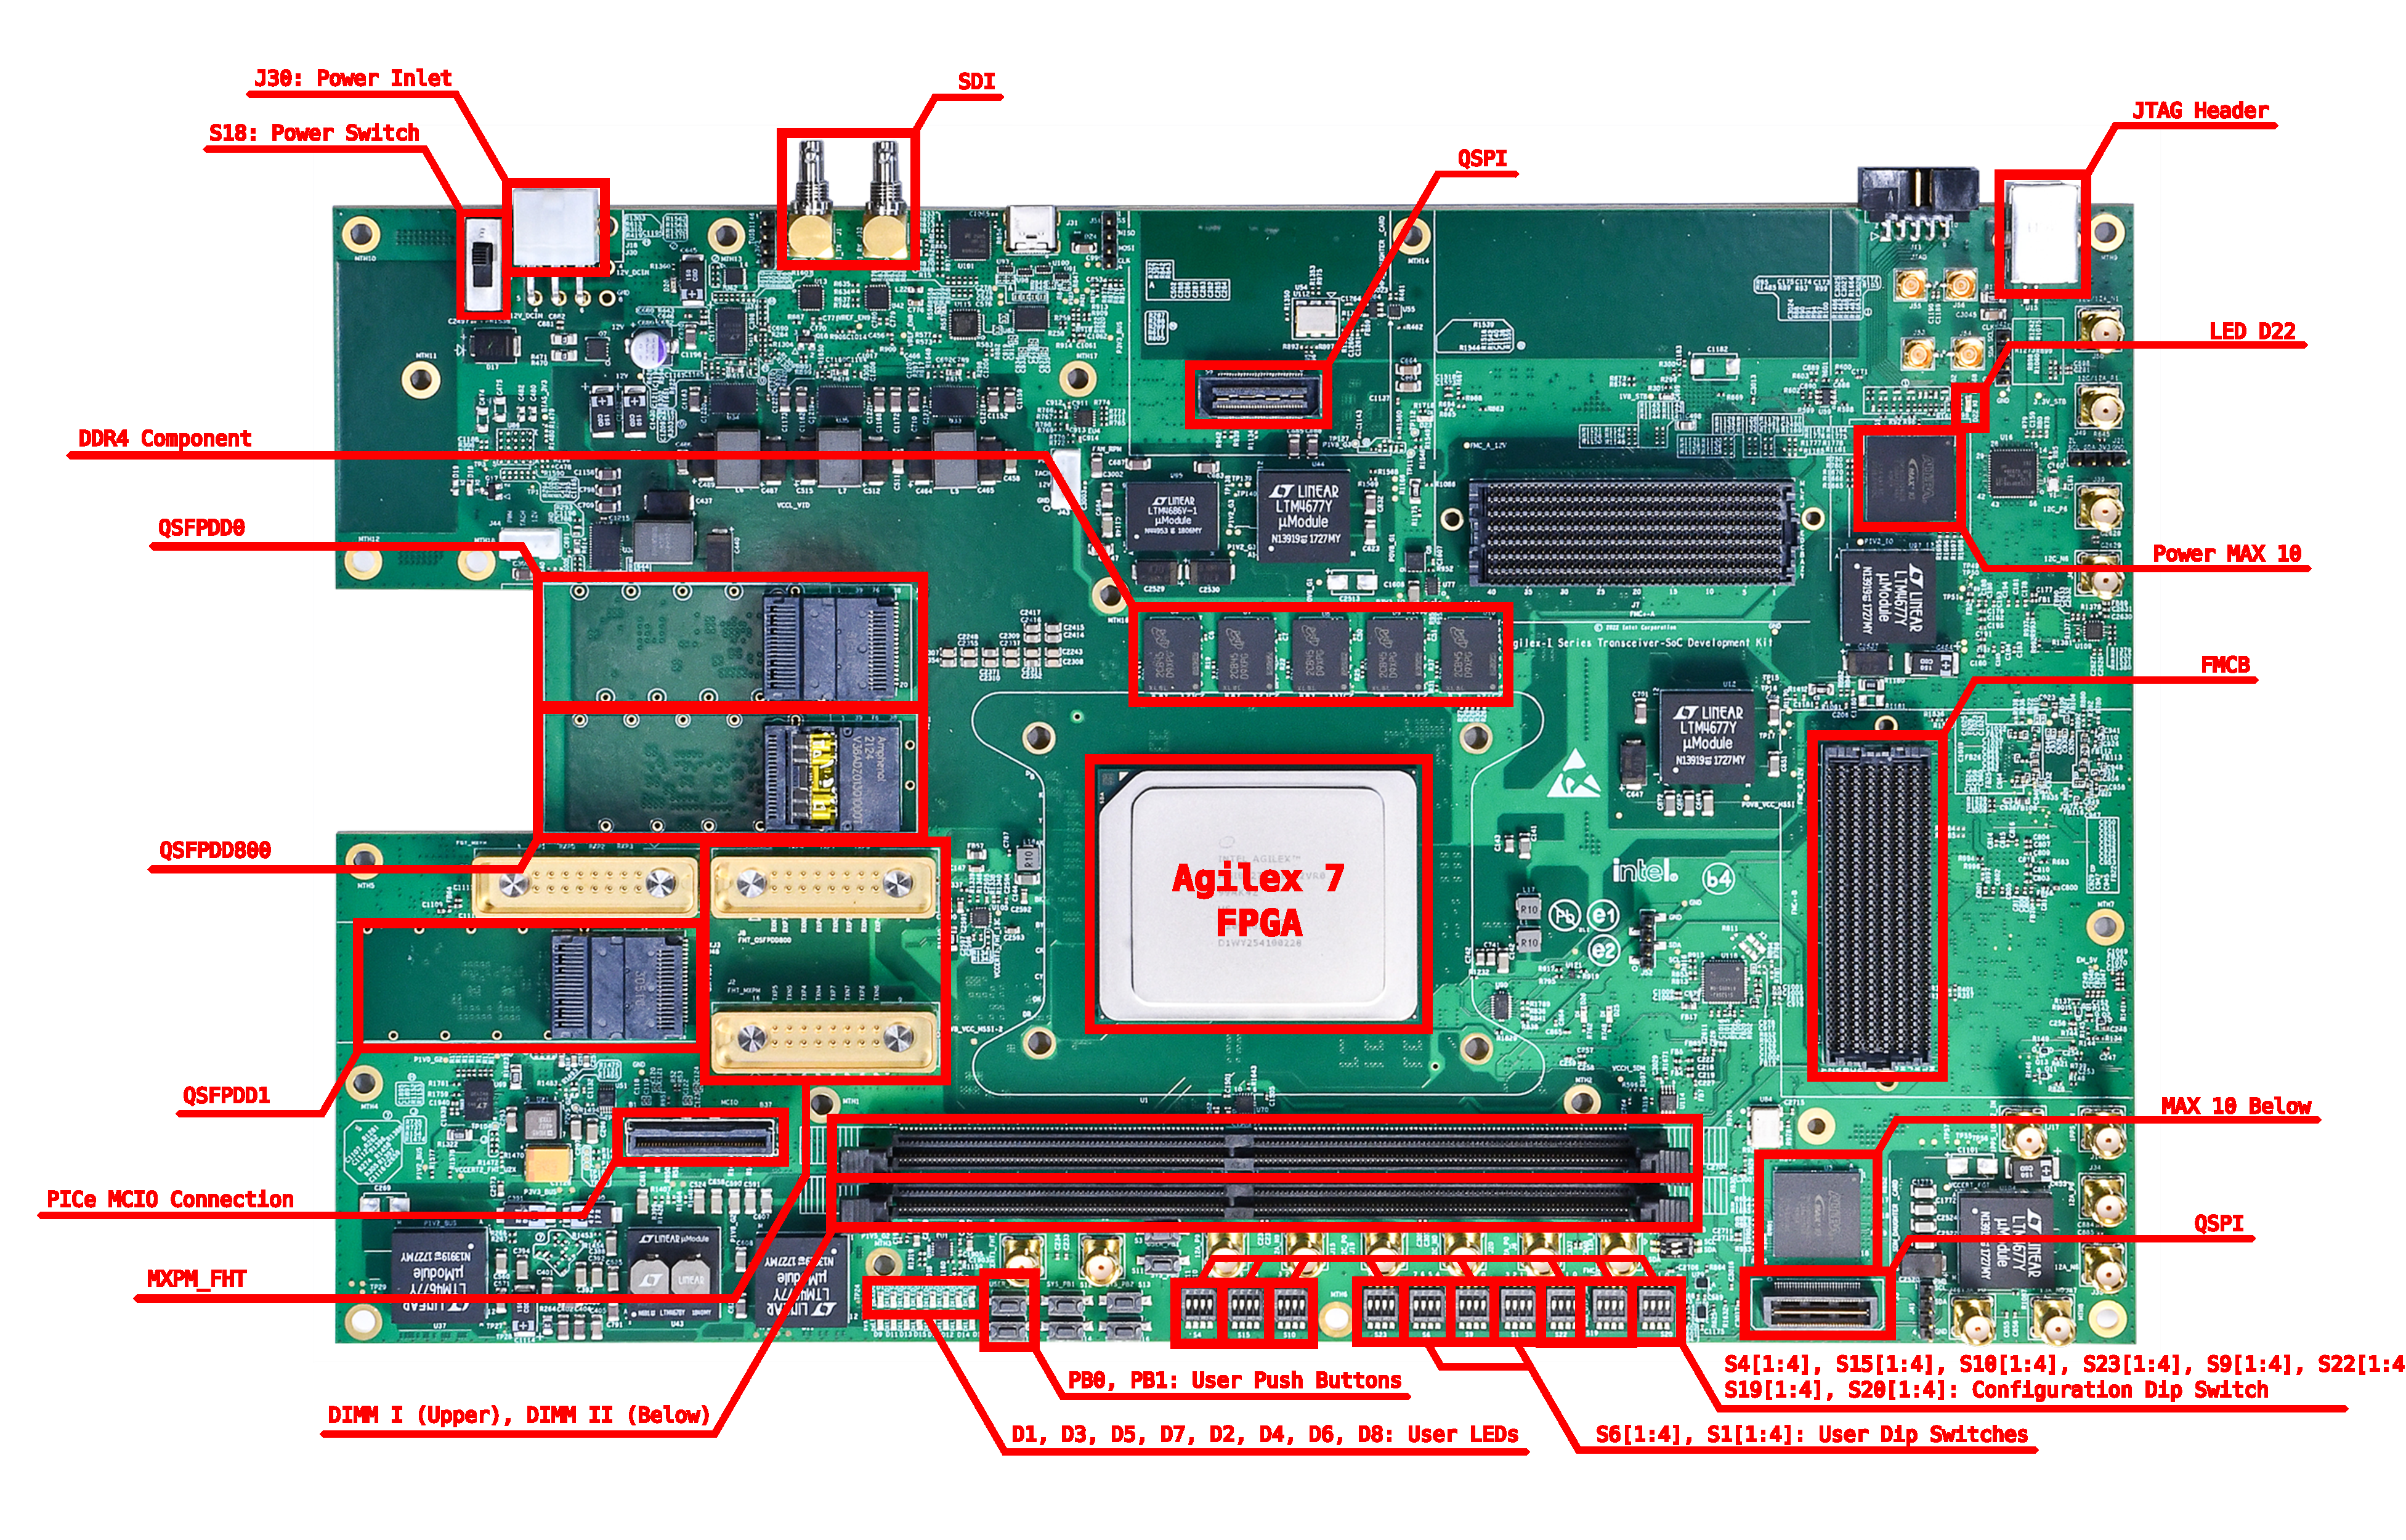
\includegraphics[width=\linewidth]{Images/Parte1/agilex7label.pdf}
        \caption{Elementos que integran a la tarjeta de desarrollo.}
        % \label{fig:enter-label}
    \end{figure}

\subsection{Resumen de caracter\'isticas}

\begin{itemize}
    \item Agilex 7 FPGA I-Series, 2.7M LE, 3184B package
    \begin{itemize}
        \item 2.7 millones de elementos l\'ogicos.
        \item Empaque tipo Ball Grid Array con 3184 bolas.
    \end{itemize}

    La tarjeta inlcuye m\'ultiples bancos de transceptores de alta velocidad (F-Tiles), dividididos en FHT y FGT.
    
    \item F-Tile 1 (13C)
    \begin{itemize}
        \item 4 canales transceptores FHT (F-Tile High-speed Transceiver) a QSFPDD800: transceptores para m\'odulos de fibra \'optica Quad Small Form-Factor Pluggable Double Density 800 (hasta 800 Gbps).
        \item 8 canales transceptores FGT (F-Tile General-purpose Transceiver) a QSFPDD: transceptores m\'as comunes, conectados a m\'odulos \'opticos QSFPDD.
        \item 2 canales transceptores FGT a HD-BNC: transmisi\'on de video (Serial Digital Interface).
        \item 4 transceptores FGT a DP2.0: Salida para DisplayPort 2.0.
        \item 1 transceptor FGT a USB3.2: Interfaz USB de alta velocidad.
    \end{itemize}
    \item F-Tile 2 (13A)
    \begin{itemize}
        \item 4 canales transceptores FHT (116G) a MXPM (Multi CoaX Press Mount): conectores de alta densidad para pruebas o backplanes.
        \item 8 canales transceptores FGT (56G) a MXPM.
        \item 8 canales transceptores FGT a QSFPDD.
        \item 4 canales transceptores FGT a MCIO (PCIe): interfaz PCI Express usando est\'andar Multi-Connector I/O.
    \end{itemize}
    \item F-Tile 3 (12C)
    \begin{itemize}
        \item 16 canales FGT a FMC+: permite conectar daughter cards por medio del est\'andar FPGA Mezzanine Card Plus para ampliar la funcionalidad.
    \end{itemize}
    \item F-Tile 4 (12A) 
    \begin{itemize}
        \item 16 canales FGT a FMC+.
    \end{itemize}
    \item SR DDR4 2666 (x72 w/ECC), 16 GB
    \begin{itemize}
        \item Memoria RAM DDR4 de 16 GB con Error Correcting Code y soporte para configuraciones de double rank (2DPC).
    \end{itemize}
    \item 8 GB SR DDR4-2666 (x72 w/ECC) dedicada al HPS.
    \item Interfaz IO48 para HPS Out of Box Experience (OOBE) daughter cards
    \begin{itemize}
        \item Intefaz de 48 pines para conectar tarjetas de desarrollo o pruebas r\'apidas del subsitema HPS.
    \end{itemize}
\textit{Nota: para m\'as informaci\'on sobre el HPS digirse a la secci\'on \hyperref[hpssec]{Hard Processor System (HPS)}}.
\end{itemize}

\subsection{Contenidos de la caja}

\begin{itemize}
    \item Agilex 7 FPGA I-Series Transceiver-SoC Development Kit
\item Modulo de memoria DDR4 DIMM (Single-rank)
\item QSPI flash daughter card: tarjeta secundaria con memoria flash QSPI preprogramada con im\'agenes de f\'abrica para configurar la FPGA.
\item HPS IO48 OOBE daughter card: Tarjeta secundaria que incluye interfaces Ethernet, USB, UART y GPIO para facilitar la evaluaci\'on del HPS.
\item NAND daughter card: Tarjeta secundaria con memoria NAND flash utilizada para almacenamiento adicional o configuraci\'on alternativa.
\item Cable USB 2.0 tipo B 
\item Cable Ethernet 
\item Fuente de alimentaci\'on de 240W y cables NA/EU/JP/UK 
\item Adaptador para fuente de poder ATX - 24 pines a 6 pines
\end{itemize}

    \begin{figure}[H]
        \centering
        \begin{subfigure}[b]{0.4\linewidth}
            \centering
            \includegraphics[width=\linewidth]{Images/Parte1/qspiflash.png}
            \caption{QSPI Flash Card.}
            % \label{sourcefpga}
        \end{subfigure} \hspace{1cm}
        \begin{subfigure}[b]{0.4\linewidth}
            \centering
            \includegraphics[width=\linewidth]{Images/Parte1/nandcard.png}
            \caption{NAND daughter card.}
            % \label{sourcefpga}
        \end{subfigure}
        \caption{Tarjetas hijas externas.}
        % \label{fig:enter-label}
    \end{figure}

\subsection{Condiciones de operaci\'on recomendadas}

\begin{table}[H]
    \centering
    \begin{tabularx}{\linewidth}{l|X}
        \toprule 
        \multicolumn{1}{c}{\textbf{Condición de operación}} & \multicolumn{1}{c}{\textbf{Rango de valores}} \\
        \toprule
        Rango de operación para temperatura ambiente & $0\degree$C a $30\degree$C \\ 
        \midrule
        Carga de corriente ICC & 195 A \\
        \midrule
        Porcentaje de carga transitorio ICC & 200 $A/\mu$s \\ 
        \midrule
        FPGA Máxima potencia soportada por disipador/ventilador activo & 160 $W$\footnotemark \\ 
        \bottomrule
    \end{tabularx}
    \caption{Condiciones de operación recomendadas.}
    \label{tab:my_label}
\end{table}
\footnotetext{160 $W$ para el núcleo y 60 $W$ para el transceptor FGT.}



   \section{Encendido de la tarjeta de desarrollo}

   Cuando se est\'a sosteniendo la tarjeta de desarrollo es muy importante tomar las precauciones adecuadas para no dañarla, ya que es susceptible a las descargas electroest\'aticas. 

   \begin{description}
       \item[\textbf{\textit{\textcolor{red}{Precauci\'on:}}}] La tarjeta puede ser dañada sin el manejo anti-descargas adecuado. Además, se deben usar precauciones anti-est\'atica cuando se toca la tarjeta.
       \item[\textbf{\textit{\textcolor{red}{Precauci\'on:}}}] Esta tarjeta de desarrollo no debe ser operada en un ambiente vibratorio.
   \end{description}

\subsection{Configuraci\'on de la tarjeta de desarrollo}

    Las instrucciones de esta secci\'on explican c\'omo configurar la tarjeta de desarrollo para el uso en casos espec\'ificos.

\subsection{Configuraci\'on predeterminada}

    La tarjeta de desarrollo Agilex 7 FPGA I-Series trae incluidos switches preconfigurados para soportar los ejemplos de diseño en el kit. Si se sospecha que la tarjeta de desarrollo no está configurada correctamente, sigue las instrucciones de la \ctref{tablasw} para regresar a la configuraci\'on predeterminada antes de avanzar.

    \begin{description}
        \item[\textit{Nota:}] ``X'' significa No Importa en la \ctref{tablasw}. 
        \item[\textit{Nota:}] No se deben de cambiar los switches de configuraci\'on cuando la tarjeta est\'a encendida, solamente cuando est\'a apagada.
    \end{description}

  \begin{longtable}{p{0.15\linewidth}|p{0.25\linewidth}|p{0.5\linewidth}} 
% \caption{Configuraci\'on por defecto de los switches de configuraci\'on.}
%   \label{tablasw}\\
            \toprule
             \multicolumn{1}{c}{\textbf{Switch}}&\multicolumn{1}{c}{\textbf{Posici\'on predeterminada}}&\multicolumn{1}{c}{\textbf{Funci\'on predeterminada}}\\ 
             \toprule
             \endfirsthead

            \toprule
             \multicolumn{1}{c}{\textbf{Switch}}&\multicolumn{1}{c}{\textbf{Posici\'on predeterminada}}&\multicolumn{1}{c}{\textbf{Funci\'on predeterminada}}\\ 
             \toprule
             \endhead
             
             S19[1:4]&OFF/OFF/ON/ON& Sistema Max 10 y FPGA seleccionada en la cadena JTAG. \\\midrule
             S20[1:4]&ON/ON/ON/ON& Modo 1: El circuito de descarga integrado de Intel actua como el \'unico JTAG maestro. HPS encadenado con nodos SDM internamente.\\\midrule
             S9[1:4]&ON/OFF/OFF/X&\parbox[t]{\linewidth}{Configuraci\'on de modo de carga de bits: AS - modo r\'apido.}\\\midrule
             S10[1:4]&ON/ON/ON/ON&
             \parbox[t]{\linewidth}{SYS\_SW[0:3]
             \begin{itemize}
                 \item SYS\_SW[0]-Factory Loadn
\item '0'-Load image from Page 0 of the
QSPI
\item SYS\_SW[1]-MUX\_SEL1
\item SYS\_SW[2]-MUX\_SEL7
\item SYS\_SW[3]-MUX\_SEL9\end{itemize}}\\\midrule
             S15[1:4]&ON/ON/ON/OFF&\parbox[t]{\linewidth}{SYS\_SW[4:7]
             \begin{itemize}
                 \item SYS\_SW[4]-MUX\_SEL\_ZL
\item SYS\_SW[5]-FMC-A PCIe RP/EP
Select
\begin{itemize}
    \item '0': RP (Default)
\item '1': EP
\end{itemize}
\item SYS\_SW[6]-FMC-B PCIe RP/EP
Select
\begin{itemize}
    \item '0': RP (Default)
\item '1': EP
\end{itemize}
\item SYS\_SW[7]-MCIO PCIe RP/EP
Select
\begin{itemize}
    \item '0': RP
\item '1': EP (Default)
\end{itemize}
\end{itemize}}\\\midrule

             S1[1:4]&OFF/OFF/OFF/OFF&Switch de usuario [0:3]\\\midrule
             S6[1:4]&OFF/OFF/OFF/OFF&\parbox[t]{\linewidth}{Switch de usuario [4:7]}\\\midrule
             
             S22[1:4]&ON/ON/ON/ON&\parbox[t]{\linewidth}{MUX\_DIP\_SW[0:3]
             \begin{itemize}
             \item MUX\_DIP\_SW0-MUX\_SEL2
\item MUX\_DIP\_SW1-MUX\_SEL3
\item MUX\_DIP\_SW2-MUX\_SEL4
\item MUX\_DIP\_SW3-MUX\_SEL5
             \end{itemize}}
             Puesto en ``ON'' por defecto para seleccionar el reloj integrado como entrada.
             \\\midrule
             
             S23[1:4]&ON/ON/ON/ON&
             \parbox[t]{\linewidth}{MUX\_DIP\_SW[4:7]
             \begin{itemize}
             \item MUX\_DIP\_SW4-MUX\_SEL10
\item MUX\_DIP\_SW5-MUX\_SEL11
\item MUX\_DIP\_SW6-MUX\_SEL12
\item MUX\_DIP\_SW7-MUX\_SEL14
             \end{itemize}}
             Puesto en ``0''/cerrado por defecto para el reloj integrado como entrada.
             \\\midrule
             S4[1:4]&ON/ON/ON/ON&
             \parbox[t]{\linewidth}{MUX\_DIP\_SW[8:11]
             \begin{itemize}
             \item MUX\_DIP\_SW8-MUX\_SEL13
\item MUX\_DIP\_SW9-MUX\_SEL6
\item MUX\_DIP\_SW10-MUX\_SEL0
\item MUX\_DIP\_SW11-MUX\_SEL8
             \end{itemize}}
             Puesto en ``0''/cerrado por defecto para el reloj integrado como entrada.
             \\\bottomrule

             \caption{Configuraci\'on por defecto de los switches de configuraci\'on.}
        \label{tablasw}
        \end{longtable}
        

\subsection{Encendido}

        Para el correcto encendido de la tarjeta debemos realizar los siguientes pasos:
        \begin{enumerate}
            \item Usa el adaptador de alimentaci\'on de 240 $W$ para suministrar alimentaci\'on a trav\'es de \texttt{\textcolor{red}{J30}}.
            \item Despu\'es de que el adaptador de alimentaci\'on est\'a conectado en \texttt{\textcolor{red}{J30}} y el switch \texttt{\textcolor{red}{S18}} est\'a en la posici\'on de ON el LED \texttt{\textcolor{red}{D22}} se enciende, indicando que la tarjeta se encendio correctamente. Si el LED \texttt{\textcolor{red}{D22}} no se enciende, significa que una o m\'as fuentes de alimentaci\'on son incorrectas.
        \end{enumerate}
        \textit{Nota: Al encender la tarjeta los ventiladores generan bastante ruido, sin embargo esto es normal y no debe generar preocupaci\'on}.
    
        \begin{figure}[H]
            \centering
            \begin{subfigure}[b]{0.4\linewidth}
                \centering
                \includegraphics[width=\linewidth, clip, trim=7cm 6cm 7cm 4cm ]{sourcefpga.png}
                \caption{Entrada de alimentaci\'on a el FPGA.}
                \label{sourcefpga}
            \end{subfigure}
            \hspace{.5cm}
            \begin{subfigure}[b]{0.4\linewidth}
                \centering
                \includegraphics[width=\linewidth, clip, trim=9cm 7cm 7cm 4.5cm ]{jtagfpga.png}
                \caption{Conexi\'on USB JTAG para el programador.}
                \label{jtagfpga}
            \end{subfigure} 

            
            \begin{subfigure}[b]{0.4\linewidth}
                \centering
            \includegraphics[width=\linewidth, clip, trim=13cm 8cm 7cm 6cm]{switch.png}
            \caption{Posici\'on de apagado para el switch de encendido.}
            \label{fig:switch}
            \end{subfigure}
            
            \caption{Conexi\'on de alimentaci\'on y USB JTAG a la tarjeta y encendido de la tarjeta.}
            \label{fig:conexion}
        \end{figure}

\section{Reinicio de la tarjeta de desarrollo}

    Esta tarjeta de desarrollo inicia con los diseños de ejemplo \curl{bts_config} almacenadas en el dispositivo de memoria flash QSPI. El proceso de reinciar la tarjeta a su configuraci\'on de f\'abrica consiste en grabar el contenido original en el MAX 10, que supervisa el sistema, y la memoria flash QSPI, donde se guarda la configuraci\'on de arranque del FPGA.\\ 
    
    Se puede realizar el reinicio de la tarjeta siguiendo las siguientes instrucciones a trav\'es de la interfaz Quartus Prime Programmer GUI.

\subsection{Reiniciar el MAX 10 con la im\'agen de f\'abrica}

El MAX 10 es un FPGA que controla el encendido del sistema, JTAG, monitoreo de voltajes, entre otras funciones. Para grabar los contenidos originales hay que seguir los siguientes pasos.

\begin{enumerate}
    \item Abrir Quartus Prime Programmer GUI y detectar la cadena JTAG despu\'es de que System MAX 10 es almacenado.
    \item Adjunta la imagen de System MAX 10 en la parte System MAX 10.
    \item Seleccionar opciones de programaci\'on y dar click en el bot\'on de programar.
\end{enumerate}

\textit{Nota: Una vez que se conecta el cable de descarga FPGA entre} \texttt{\textcolor{red}{J11}} \textit{y la estaci\'on de trabajo, se desactiva autom\'aticamente el circuito de descarga integrado en la placa.}

\subsection{Reinicio de la memoria flash QSPI con la imagen de f\'abrica}

    La memoria flash QSPI est\'a pre-programada con 4 paquetes de im\'agenes. Los pasos siguientes indican como sobreescribir la imagen de modo de configuraci\'on de la interfaz de transmisi\'on Avalon x8.

    \begin{enumerate}
        \item Asegurarse que MSEL[2:0] est\'a apagado (modo JTAG) antes de encender la tarjeta.
        \item Abrir Quartus Prime Programmer GUI y detectar la cadena JTAG.
        \item Cambiar el dispositivo VTAP10 a 10M50DAF256, adjuntar el dispositivo flash de QSPI\_2Gb.
        \item Adjuntar el archivo de configuraci\'on para el modo Avalon Streaming interface x8 a QSPI\_2Gb.
        \item Seleccionar las opciones Programar/Configurar y dar click en el bot\'on \texttt{\textcolor{DarkOrchid1}{Start}}.
        \item Despu\'es de programar la memoria flash apagar la tarjeta y cambiar MSEL[2:0] OFF OFF ON (modo de configuraci\'on por Avalon Streaming interface x8).
    \end{enumerate}
%     \chapter{Board Test System}

El FPGA Agilex 7 I-Series Transceiver-SoC Development Kit incluye diseños de ejemplo y la GUI Board Test System (BTS) para probar el funcionamiento de la tarjeta. Este software provee una interfaz fácil de usar para alterar la configuración funcional y observar los resultados. Además, se puede utilizar para probar y verificar el funcionamiento de componentes (DDR4, QSPI, USB, PCIe, FMC, trasceptores, etc.), modificar parámetros funcionales (frecuencia, voltaje, modo del transceptor, etc.), observar el rendimiento y medir el consumo de energía por bloque o interfaz. 

Mientras se est\'a usando el BTS se realiza una reconfiguraci\'on del FPGA varias veces con diseños de prueba específicos para la funcionalidad que se está probando. El BTS también es útil como referencia para diseño de sistemas. El BTS se comunica a través del puerto JTAG a un diseño de pruebas ejecutandose en la tarjeta de desarrollo.

\begin{figure}[H]
        \centering
        \includegraphics[width=0.6\linewidth]{image2.png}
        \caption{BTS GUI.}
        \label{fig:image2}
    \end{figure}



\section{Ejecuci\'on del Board Test System}

        Para abrir el \bts (BTS) tenemos que seguir los siguientes pasos. 

        \begin{enumerate}
            \item Conectar el cable USB2.0 tipo B de la tarjeta a la estaci\'on de trabajo.
            \item Revisar que la configuraci\'on de la tarjeta sea correcta. En la mayor\'ia de los casos el BTS requiere que el MAX 10 y el FPGA Agilex 7 est\'en en la cadena JTAG, mientras que el Controlador del Reloj y el Monitor de Energ\'ia solo requiere el MAX 10.
            \item Revisa el estatus de los m\'odulos externos: cable MXPM/QSFP/QSFPDD/FMC/DIMM
            \item Enciende la tarjeta.
            \item En la estaci\'on de trabajo, en una nueva terminal ejecutar el comando \texttt{\textcolor{blue}{bts}}.
        \end{enumerate}

        \begin{figure}[H]
            \centering
            \includegraphics[width=0.6\linewidth]{terminal1.png}
            \caption{Comando de ejecuci\'on para lanzar el BTS.}
            \label{terminal1}
        \end{figure}

        Cuando se ejecuta el BTS aparece inicialmente una pequeña ventana que indica que el software se ejecut\'o correctamente y se est\'a preparando para lanzarse (\cref{fig:image1}), o bien una ventana de error que indica que la tarjeta no est\'a conectada (\cref{fig:image10}). Después de un momento se muestra la GUI del BTS (\cref{fig:image2}).

    \begin{figure}[H]
        \centering
        \begin{subfigure}[c]{0.4\linewidth}
            \includegraphics[width=\linewidth]{image1.png}
            \caption{Ventana de preparaci\'on de lanzamiento para el BTS.}
        \label{fig:image1}
        \end{subfigure} \hspace{.5cm}
        \begin{subfigure}[c]{0.45\linewidth}
        \centering
        \includegraphics[width=\linewidth]{image10.png}
        \caption{Ventana de error al ejecutar el BTS.}
        \label{fig:image10}
        \end{subfigure}
        \caption{Casos que se presentan al ejecutar \texttt{\textcolor{blue}{bts}} desde terminal.}
    \end{figure}

    \begin{figure}[H]
        \centering
        \includegraphics[width=0.6\linewidth]{image2.png}
        \caption{Ventana inicial del BTS.}
        \label{fig:image2}
    \end{figure}

\subsection{Inicializaci\'on de variables}
        
    \textcolor{blue}{\textit{Nota: Lo que se explica en esta secci\'on solamente es el funcionamiento del comando} \texttt{bts}\textit{, el cual es una simplificaci\'on del proceso normal para abrir el BTS.}}

    Para inicializar las variables que requiere el BTS se modifica el archivo \curl{~/.bashrc} para que exporte las variables contenidas en el archivo \curl{~/Desktop/Variables\_BTS.txt}, que es donde se almacenan las variables de entorno.
    
\begin{lstlisting}[language=bash, label=cod1]    
#Variables de entorno para inicializar el BTS

export QSYS_ROOTDIR=/home/liese2/intelFPGA_pro/24.3.1/qsys/bin
export QUARTUS_ROOTDIR=/home/liese2/intelFPGA_pro/24.3.1/quartus\end{lstlisting}
    Despu\'es de establecer estas variables se debe ejecutar el archivo \curl{/home/liese2/Documents/agilex-agib027r31b1e1vb-si-nen-revc-v24-3b194-v1-0/examples/board\_test\_system/BoardTestSystem.sh}. 

    % \begin{figure}[H]
    %     \centering
    %     \includegraphics[width=0.6\linewidth]{terminal2.png}
    %     \caption{Instrucciones necesarias para lanzar el BTS de forma normal.}
    %     \label{terminal2}
    % \end{figure}

    Para ahorrarnos estos pasos se agrega la siguiente linea en el archivo \curl{~/.bashrc}:

\begin{lstlisting}[language=bash, label=cod1]
alias bts='source ~/Desktop/Variables_BTS.txt && cd /home/liese2/Documents/agilex-agib027r31b1e1vb-si-nen-revc-v24-3b194-v1-0/examples/board_test_system && ./BoardTestSystem.sh'\end{lstlisting}

\textit{Nota:} Para modificar el archivo \curl{~/.bashrc} se debe ejecutar el siguiente comando en una terminal, aunque se recomienda no realizar ninguna modificaci\'on.
\begin{lstlisting}[language=bash, label=cod1]
sudo nano ~/.bashrc\end{lstlisting}


\section{Probando el BTS.}

\subsection{Informaci\'on del borde inferior}   

    La barra de informaci\'on del borde inferior muestra el estatus de la conexi\'on, la versi\'on de Quartus Prime y el reloj JTAG.

    \begin{description}
        \item[System Connected/Disconnected:] Muestra si la tarjeta est\'a conectada a la estaci\'on de trabajo. Si la tarjeta se desconecta la señal verde se vuelve gris.
        \item[Quartus Prime Version:] Muestra la versi\'on actual de Quartus Prime instalada en la estaci\'on de trabajo. El texto se vuelve rojo si la versi\'on actual es m\'as antigua que la versi\'on requerida. Si se tiene instalada la versi\'on correcta pero la versi\'on activa no cumple los requisitos cambia la variable de entorno \texttt{\textcolor{blue}{QUARTUS\_ROOTDIR}}.
        \item[JTAG:] Muestra la frecuencia del reloj JTAG.
    \end{description}

    \begin{figure}[H]
        \centering
        \includegraphics[width=0.7\linewidth, clip, trim={0 0 0 19cm}]{image2.png}
        \caption{Informaci\'on del borde inferior del BTS.}
        \label{fig:image2}
    \end{figure}


\subsection{Men\'u de configuraci\'on}

    Usa el men\'u de configuraci\'on para seleccionar el diseño que se va a utilizar. Cada diseño de ejemplo prueba diferentes funcionalidades que corresponden a una o a m\'as pestañas de aplicación.

    \begin{figure}[H]
        \centering
        \includegraphics[width=0.6\linewidth]{image3.png}
        \caption{Opciones de configuraci\'on para la tarjeta.}
        % \label{fig:image3}
    \end{figure}

    Para configurar la FPGA con un diseño de prueba se realiza lo siguiente:

    \begin{enumerate}
        \item En el men\'u \texttt{\textcolor{DarkOrchid1}{Configure}} dar click a la opci\'on que corresponde a la funcionalidad que se quiere probar.
        \item En la ventana del programador que aparece, dar click en \texttt{\textcolor{DarkOrchid1}{Configure}} para descargar el archivo SRAM Object File (\texttt{\textcolor{blue}{.sof}}) correspondiente a la FPGA. Este proceso usualmente tarda menos de un minuto.
        \item Cuando la configuraci\'on termina, el diseño empieza a ejecutarse en la FPGA. La pestaña correspondiente a la aplicación que nos permite interactuar con el diseño se habilita en la GUI. Si se us\'o Quartus Prime Programmer para la configuraci\'on, en vez de la BTS GUI, puede que sea necesario reiniciar la GUI.
    \end{enumerate}

\subsubsection{Ejemplo usando el diseño de prueba para GPIO.}

    Siguiendo los pasos anteriores, en el menú de configuración seleccionaremos la opci\'on \texttt{\textcolor{DarkOrchid1}{Configure with GPIO Design}}, al seleccionar se abre una ventana del programador (\cref{fig:image4}), en la cual simplemente se tiene que dar click en el bot\'on \texttt{\textcolor{DarkOrchid1}{Configure}}. En este caso nos apareció un error propio de la GUI que indica que se tiene que reinciar el BTS (\cref{fig:image5}).

    \begin{figure}[H]
        \centering
        \begin{subfigure}[c]{0.4\linewidth}
        \includegraphics[width=\linewidth]{image4.png}
        \caption{Programador para el primer ejemplo.}
        \label{fig:image4}
        \end{subfigure}\hspace{.5cm}
        \begin{subfigure}[c]{.45\linewidth}
        \centering
        \includegraphics[width=\linewidth]{image5.png}
        \caption{Error que se lanza cuando el programador termina de configurarse.}
        \label{fig:image5}
        \end{subfigure}
        \caption{Cargador del programa y error al completarse.}
    \end{figure}

     Para reiniciar la GUI seleccionamos en el menú de configuración \texttt{\textcolor{DarkOrchid1}{Exit}} y volvemos a ejecutar el comando \texttt{\textcolor{blue}{bts}} en terminal.

    % \begin{figure}[H]
    %     \centering
    %     \includegraphics[width=0.6\linewidth]{image6.png}
    %     \caption{Instrucci\'on para salir del BTS.}
    %     \label{fig:image6}
    % \end{figure}
    
    % \begin{figure}[H]
    %     \centering
    %     \includegraphics[width=0.6\linewidth]{image7.png}
    %     \caption{Relanzamiento del BTS.}
    %     \label{fig:image7}
    % \end{figure}

    Cuando el BTS se lanza nuevamente, ahora aparece una interfaz diferente, ya que se habilita la pestaña de \textit{GPIO}, el cual muestra el programa configurado anteriormente (\cref{fig:image8}) que nos permite observar los cambios en los puertos I/O de usuario (LED's, dip-switches y push-buttons). Adem\'as, podemos darnos cuenta de que el programa se carg\'o correctamente al observar que en el FPGA se encendieron los LED's de usuario (\cref{fig:image11}). Tanto en el BTS como en la tarjeta se muestran los LED's de usuario numerados del 0 al 7.

    \begin{figure}[H]
        \centering
        \includegraphics[width=0.6\linewidth]{image8.png}
        \caption{Programa cargado al ejecutar \textit{Configure with GPIO Design}.}
        \label{fig:image8}
    \end{figure}

    \begin{figure}[H]
        \centering
        \includegraphics[width=0.5\linewidth, clip, trim=5cm 5cm 12cm 9cm]{image11.png}
        \caption{LED's de usuario que se encienden al cargar el programa.}
        \label{fig:image11}
    \end{figure}

    Podemos hacer click sobre los íconos de LED's mostrados en el BTS para encenderlos o apagarlos y esto se ver\'a reflejado en la tarjeta. De igual forma, al modificar en la tarjeta la posición de los dip-switches o presionar los push-button esto se refleja en la GUI.

    \begin{figure}[H]
        \centering
        \includegraphics[width=0.6\linewidth]{image9.png}
        \caption{Modificaci\'on del estado de los LED's de usuario desde el BTS.}
        \label{fig:image9}
    \end{figure}
    \begin{figure}[H]
        \centering
        \includegraphics[width=0.5\linewidth]{image12.png}
        \caption{Respuesta en los LED's de usuario en la tarjeta a los cambios realizados en el BTS.}
        \label{fig:image12}
    \end{figure}

\subsection{Pestaña de información del sistema}

    La pestaña de información del sistema muestra información acerca de la configuración actual de la tarjeta. En la pestaña se despliega la información de la tarjeta, los dispositivos de la cadena JTAG y otros detalles almacenados en la tarjeta.

    \begin{figure}[H]
        \centering
        \includegraphics[width=0.6\linewidth]{Images/Parte2/systab.png}
        \caption{Pestaña de información de la tarjeta.}
        \label{fig:systab}
    \end{figure}

    Las siguientes secciones describen los controles en la pestaña de información del sistema.

\subsubsection{Informaci\'on de la tarjeta}

    El control de informaci\'on de la tarjeta muestra informaci\'on est\'atica acerca de la tarjeta.

    \begin{itemize}
        \item \textbf{Board Name:} Indica el nombre oficial de la tarjeta dado por el BTS.
        \item \textbf{Board Revision:} Indica la revisi\'on de la tarjeta.
        \item \textbf{MAX Version:} Indica la versi\'on del sistema MAX 10.
    \end{itemize}

\subsubsection{Cadena JTAG}

    El control de la cadena JTAG muestra todos los dispositivos conectados actualmente a la cadena JTAG. 

    Se deben poner el MAX 10 y la FPGA en la cadena JTAG cuando se está ejecutando el BTS.

\subsection{Pestaña de GPIO}

    La pestaña GPIO nos permite interactuar con todos los componentes de propósito general E/S en la tarjeta. Se pueden encender o apagar los LEDs y observar el estatus de los push buttons y los dip switches.

    \begin{figure}[H]
        \centering
        \includegraphics[width=0.6\linewidth]{Images//Parte2/gpiotab.png}
        \caption{Pestaña GPIO.}
        \label{fig:enter-label}
    \end{figure}

    La siguientes secciones describen los controles en la pesta\n a GPIO.

\begin{description}
    \item[LEDs de usuario:] 
    El control de LEDs de usuario muestra el estado actual de los LEDs de usuario. Al dar click en los botones de los LEDs se puede encender o apagar los LEDs de la tarjeta. El bot\'on \texttt{\textcolor{DarkOrchid1}{All}} sirve para modificar el estado de todos los LEDs.
    \item[Dip switches de usuario:]
    El control de los dip switches de usuario muestra el estado de los switches \texttt{\textcolor{red}{USER\_SW[0:3](S1)}} y \texttt{\textcolor{red}{USER\_SW[4:7](S6)}}.
    \item[Push buttons:]
    El control de los push buttons muestra el estado de \texttt{\textcolor{red}{PB0}} y \texttt{\textcolor{red}{PB1}}
    \item[Qsys Memory Map:]
    El control Qsys Memory Map muestra el mapa de memoria del dise\n o \texttt{\textcolor{blue}{bts\_config.sof}} ejecut\'andose en la tarjeta.
\end{description}


\subsection{Pesta\n a XCVR}

    La pesta\n a XCVR permite realizar pruebas de transreceptores en la tarjeta de desarrollo. Se pueden realizar las pruebas ya sea usando un m\'odulo de loopback el\'ectrico o m\'odulos de fibra \'optica.

\subsubsection{La pesta\n a QSFPDD NRZ}

    \begin{figure}[H]
        \centering
        \includegraphics[width=0.5\linewidth]{Images//Parte2/qsfpddnrz.png}
        \caption{La pesta\n a QSFPDD NRZ.}
        % \label{fig:enter-label}
    \end{figure}

    Las siguientes secciones describen los controles en la pesta\n a QSFPDD.

    \paragraph{Estado}

        El control de estado muestra la siguiente informaci\'on durante la prueba de loopback:

        \begin{itemize}
            \item \textbf{PLL lock:} Muestra el estado de PLL bloqueado o desbloqueado.
            \item \textbf{Pattern Sync:} Muestra el patr\'on de estado sincronizado o no sincronizado. El patr\'on se considera sincronizado cuando se detecta el inicio de la secuencia de datos.
            \item \textbf{Detail:} Muestra el patr\'on de estado de sincronizaci\'on de cada canal. Tambi\'en muestra el n\'umero de bits de error de cada canal.
        \end{itemize}

        \begin{figure}[H]
            \centering
            \includegraphics[width=0.5\linewidth]{Images//Parte2/status.png}
            \caption{QSFPDD NRZ - PLL and Pattern Status.}
            % \label{fig:enter-label}
        \end{figure}

    \paragraph{Control}

        Se deben de usar los siguientes controles para seleccionar una interfaz para aplicar la configuraci\'on PMA, tipo de dato y control de error:

        \begin{itemize}
            \item QSFPDD0 x8
            \item QSFPDD1 x8
        \end{itemize}

    \paragraph{Configuraci\'on PMA}

        Permite realizar cambios a los par\'ametros PMA que afectan la interfaz del transceptor activo. Los siguientes ajustes est\'an disponibles para an\'alisis:

        \begin{itemize}
            \item \textbf{Serial Loopback:} Muestra la se\n al de estado entre el transmisor y el receptor.
            \item \textbf{VOD:} Especifica la salida de voltaje diferencial del buffer del transmisor.
            \item \textbf{Pre-emphasis tap:} 
            \begin{itemize}
                \item Pre-tap 1: Especifica la cantidad de pre\'enfasis de la primera pre-tap del buffer del transmisor.
                \item Pre-tap 2: Especifica la cantidad de pre\'enfasis en la segunda pre-tap del buffer del transmisor.
                \item Post-tap 1: Especifica la cantidad de pre\'enfasis en la post-tap del buffer del transmisor.
            \end{itemize}
        \end{itemize}

        \begin{figure}[H]
            \centering
            \includegraphics[width=0.4\linewidth]{Images//Parte2/pmasett.png}
            \caption{QSFPDD NRZ - PMA setting.}
            \label{fig:pmaset}
        \end{figure}
    
    \paragraph{Tipo de dato}

        El control de tipo de dato especifica el tipo de patr\'on de datos contenido en las transacciones. Se debe seleccionar alguno de los siguientes tipos de dato para an\'alisis:

        \begin{itemize}
            \item \textbf{PRBS7:} secuencias binarias pseudo-aleatorias de 7 bits .
            \item \textbf{PRBS15:} secuencias binarias pseudo-aleatorias de 15 bits.
            \item \textbf{PRBS23:} secuencias binarias pseudo-aleatoria de 23 bits.
            \item \textbf{PRBS32:} secuencias binarias pseudo-aleatoria de 31 bits (predeterminado).
        \end{itemize}

    \paragraph{Control de error}

        Este control muestra errores de datos detectados durante el an\'alisis y nos permite inyectar errores.

        \begin{itemize}
            \item \textbf{Detected Errors:} Muestra el n\'umero de errores de datos detectados en la transmisi\'on de datos.
            \item \textbf{Inserted Errors:} Muestra el n\'umero de errores insertados en el flujo de transmisi\'on de datos.
            \item \textbf{Bit Error Rate:} Calcula la tasa de bits de error en el flujo de transmisi\'on de datos.
            \item \textbf{Insert:} Inserta un error de una palabra en el flujo de transmisi\'on de datos cada vez que se da click en el bot\'on. La inserci\'on de errores solo se habilita durante el an\'alisis de rendimiento de transacci\'on.
            \textbf{Clear:} Resetea el contador de errores detectados y el contador de errores insertados a cero.
        \end{itemize}

    \paragraph{Control de ejecuci\'on}

        \begin{itemize}
            \item \textbf{Barras de rendimiento TX y RX:} muestra el porcentaje de la m\'axima tasa de datos te\'orica que las transacciones solicitadas pueden llegar a alcanzar.
            \item \textbf{Start:} Este control inicia el test de loopback.
            \item \textbf{Data rate:} Muestra el tipo XCVR y la tasa de datos de cada canal.
        \end{itemize}

        \begin{figure}[H]
            \centering
            \includegraphics[width=0.4\linewidth]{Images//Parte2/datarate.png}
            \caption{QSFPDD NRZ - Data Rate.}
            % \label{fig:enter-label.}
        \end{figure}

\subsubsection{La pesta\n a QSFPDD PAM4}

    Esta pesta\n a tiene funciones de control similares a la pesta\n a QSFPDD NRZ.

    \begin{figure}[H]
        \centering
        \includegraphics[width=0.5\linewidth]{Images//Parte2/qsfpddpam4.png}
        \caption{La pesta\n a QSFPDD PAM4.}
        % \label{fig:enter-label}
    \end{figure}

\subsubsection{La pesta\n a FMCA NRZ}

    Esta pesta\n a tiene funciones de control similares a la pesta\n a QSFPDD NRZ, excepto por la selecci\'on de puertos.

    \begin{figure}[H]
        \centering
        \includegraphics[width=0.5\linewidth]{Images//Parte2/fmcanrz.png}
        \caption{La peta\n a FMCA NRZ.}
        % \label{fig:enter-label}
    \end{figure}

\subsubsection{La pesta\n a FMCB NRZ}

    Esta pesta\n a tiene funciones de control similares a la pesta\n a QSFPDD NRZ, excepto por la selecci\'on de puertos.

    \begin{figure}[H]
        \centering
        \includegraphics[width=0.5\linewidth]{Images//Parte2/fmcbnrz.png}
        \caption{La pesta\n a FMCB NRZ.}
        % \label{fig:enter-label}
    \end{figure}

\subsubsection{La pesta\n a QSFPDD800 PAM4}

    Esta pesta\n a tiene funciones de control similares a la pesta\n a QSFPDD NRZ.

    \begin{figure}[H]
        \centering
        \includegraphics[width=0.5\linewidth]{Images//Parte2/qsfpdd800pam4.png}
        \caption{La pesta\n a QSFPDD800 PAM4.}
        % \label{fig:enter-label}
    \end{figure}

    \begin{figure}[H]
        \centering
        \includegraphics[width=0.4\linewidth]{Images//Parte2/pmasett.png}
        \caption{QSFPDD800 PAM4 - PMA Setting.}
        % \label{fig:enter-label}
    \end{figure}

    \paragraph{Ajustes PMA}

        Adem\'as de los ajustes PMA listados en la \cref{fig:pmaset}, hay ajustes adicionales disponibles para el F-Tile FHT PMA. El PMA est\'a configurado para valores predeterminados en los dise\n os PMA4.

        \begin{itemize}
            \item \textbf{Serial Loopback:} Muestra la se\n al de estado entre el transmisor y el receptor.
            \item \textbf{VOD:} Especifica la salida de voltaje diferencial del buffer del transmisor.
            \item \textbf{Pre-emphasis tap:} 
            \begin{itemize}
                \item Post-tap 2: Especifica la cantidad de pre\'enfasis de la segunda post-tap del buffer del transmisor.
                \item Post-tap 3: Especifica la cantidad de pre\'enfasis en la tercer post-tap del buffer del transmisor.
                \item Post-tap 4: Especifica la cantidad de pre\'enfasis en la cuarta post-tap del buffer del transmisor.
                \item Pre-tap 3: Especifica la cantidad de pre\'enfasis en la tercer pre-tap del buffer del transmisor.
            \end{itemize}
        \end{itemize}

    \subsubsection{La pesta\n a MXPM NRZ}

        Esta pesta\n a tiene funciones de control similares a la pesta\n a QSFPDD NRZ, excepto por la selecci\'on de puertos.

        \begin{figure}[H]
            \centering
            \includegraphics[width=0.5\linewidth]{Images//Parte2/mxpmnrz.png}
            \caption{La pesta\n a MXPM NRZ.}
            % \label{fig:enter-label}
        \end{figure}

    \subsubsection{La pesta\n a MXPM PAM4}

        Esta pesta\n a tiene funciones de control similares a la pesta\n a QSFPDD NRZ.

        \begin{figure}[H]
            \centering
            \includegraphics[width=0.5\linewidth]{Images//Parte2/mxpmpam4.png}
            \caption{La pesta\n a MXPM PAM4.}
            % \label{fig:enter-label}
        \end{figure}

    \subsection{La pesta\n a SDI}

        Esta pesta\n a tiene funciones de control similares a la pesta\n a QSFPDD NRZ.

        \begin{figure}[H]
            \centering
            \includegraphics[width=0.5\linewidth]{Images//Parte2/sdi.png}
            \caption{La pesta\n a SDI.}
            % \label{fig:enter-label}
        \end{figure}

\subsection{La pesta\n a de memoria}

    Esta pesta\n a nos permite leer y escribir en las memorias DDR4 DIMM-2A (DIMM-I) y DDR4 DIMM-2B (DIMM-II) de la tarjeta de desarrollo. RDIMMS solo realiza pruebas DIMM-II mientras que se realizan las pruebas pruebas RDIMMD DIMM-I y DIMM-II. Descarga el dise\n o a trav\'es del men\'u de configuraci\'on.

    \begin{figure}[H]
        \centering
        \includegraphics[width=0.6\linewidth]{Images//Parte2/memorytab.png}
        \caption{La pesta\n a  RDIMMS.}
        % \label{fig:enter-label}
    \end{figure}

    Las siguientes secciones describen los controles en esta pesta\n a.

\begin{description}
    \item[Start:] 
        Inicializa el an\'alisis de rendimiento de trasacci\'on de memoria DDR4.
    \item[Stop:]
        Finaliza el an\'alisis de rendimiento de transacci\'on.
    \item[Reset:]
        Reincia el an\'alisis de rendimieto de transacci\'on.
\end{description}

    \paragraph{Performance Indicators}

        Estos controles muestran la informaci\'on actual del an\'alisis de rendimiento de transacci\'on colectada desde que se dio click en \texttt{\textcolor{DarkOrchid1}{Start}}.

        \begin{itemize}
            \item \textbf{Write and Read performance bars}: Muestra el porcentaje de la m\'axima tasa de datos te\'orica que las transacciones requeridas son capaces de alcanzar.
            \item \textbf{Write (MBps) and Read (MBps):} Muestra el n\'umero de bytes analizados por segundo.
            \item \textbf{Data Bus:} 72 bits (8 bits ECC) de ancho, reloj de referencia de 166.666 MHz, y la frecuencia es 1333.33 MHz tasa de datos doble 2666.66 MT/s.
        \end{itemize}

    \paragraph{Test Control}

        \begin{itemize}
            \item \textbf{Test Size:} Se puede elegir el tama\n o de la memoria a probar. Las opciones disponibles son 64 KB, 1 MB, 16 MB, 64 MB, 256 MB, 1 GB, 4 GB, 8 GB, y 16 GB (por default).
            \item \textbf{Offset (Hex):} Se puede definir la direcci\'on de memoria de inicio para probar.
            \item \textbf{Test Mode:} Lectura y Escritura infinita (default), Lectura y Escritura singular.
            \item \textbf{Test Pattern:} PRBS (default), Constante Definida por Usuario, Walking '0', Walking '1'.
        \end{itemize}

    \paragraph{Error Control}

        Este control muestra errores de datos detectados durante el an\'alisis y te permite insertar errores.

        \begin{itemize}
            \item \textbf{Detected Errors:} Muestra el n\'umero de errores de dato detectados en el hardware.
            \item \textbf{Inserted Errors:} Muestra el n\'umero de errores insertados en la transmisi\'on de transacciones.
            \item \textbf{Insert:} Inserta un error de una palabra en el flujo de transacciones cada vez que se da click en el bot\'on. El bot\'on de inserci\'on de errores solamente se habilita durante el an\'alisis de rendimiento de transacci\'on.
        \end{itemize}

        \begin{figure}[H]
            \centering
            \includegraphics[width=0.6\linewidth]{Images//Parte2/rdimmstest.png}
            \caption{La pesta\n a RdIMMD. El tama\n o de prueba se puede establecer a 32 GB con dos RDIMMs.}
            % \label{fig:enter-label}
        \end{figure}
%     \chapter{Uso de la tarjeta con Quartus Prime Pro Edition}

\section{Pasos para cargar proyectos desde \quartus a la tarjeta}

    Para cargar un programa a la tarjeta de desarrollo desde \quartus debemos realizar el siguiente procedimiento con el fin de que se realice correctamente la comunicación mediante protocolo serial desde la MAX 10 al Agilex 7.

    \begin{enumerate}
        \item Conectar el cable USB2.0 tipo B de la tarjeta a la estaci\'on de trabajo.
        \item Revisar que la configuraci\'on de la tarjeta sea la configuraci\'on predeterminada.
        \item Revisa el estatus de los m\'odulos externos: cable MXPM/QSFP/QSFPDD/FMC/DIMM
        \item Encender la tarjeta.
        \item En la estaci\'on de trabajo abrir Quartus Prime Pro Edition
        \item Abrir el proyecto que se va a cargar a la tarjeta de desarrollo.
        \item Establecer las configuraciones necesarias para el dispositivo.
        \item Configurar el programador para que trabaje con el hardware correspondiente a la tarjeta de desarrollo.
        \item Establecer la configuraci\'on del programador e incluir los archivos necesarios.
        \item Ejecutar el proyecto en la tarjeta de desarrollo.
    \end{enumerate}

\subsection{Ejemplo de programa para hacer parpadear un LED}

    Se muestra el siguiente ejemplo que realiza la conmutaci\'on de uno de los LED's de usuario, se muestran los pasos a seguir con el fin de que la comunicaci\'on al chip Agilex 7 se establezca correctamente. 
    
    El proyecto con el cual se realizar\'a este ejemplo se encuentra en el archivo \curl{home/liese2/Proyects/blinky.qpf}, este ser\'a el archivo que nos ayudar\'a a cargar el programa funcional a la tarjeta. Al abrirlo se mostrar\'a la vista inicial del proyecto y en el \texttt{\textcolor{DarkOrchid1}{Project Navigator}} se muestran los archivos que contiene (\cref{fig:screen1}).

    % \begin{figure}[H]
    %     \centering
    %     \includegraphics[width=0.5\linewidth, clip, trim= 0 0 3cm 0]{Images//Parte3/recent.png}
    %     \caption{Proyectos recientes utilizados en \quartus.}
    %     \label{fig:recent}
    % \end{figure}
    \begin{figure}
        \centering
        \includegraphics[width=0.9\linewidth]{Images//Parte3/screen1.png}
        \caption{Vista inicial al abrir el proyecot}
        \label{fig:screen1}
    \end{figure}

    El siguiente paso ser\'a realizar ciertas configuraciones: para ello debemos ir a \texttt{\textcolor{DarkOrchid1}{{Assignments $\rightarrow$ Device $\rightarrow$ Device and Pin Options}}} (\cref{fig:configgen}) para realizar dos configuraciones.
    
    La primera de ellas es en \texttt{\textcolor{DarkOrchid1}{Configuration $\rightarrow$ Configuration Pin Options}}, dentro de este menú se deben marcar las opciones \texttt{\textcolor{DarkOrchid1}{USE PWRMGT\_SCL output}}, \texttt{\textcolor{DarkOrchid1}{USE PWRMGT\_SDA output}} y \texttt{\textcolor{DarkOrchid1}{USE CONF\_DONE output}}. Además de seleccionar \texttt{\textcolor{DarkOrchid1}{SDM\_IO0}}, \texttt{\textcolor{DarkOrchid1}{SDM\_IO12}} y \texttt{\textcolor{DarkOrchid1}{SDM\_IO16}} en las respectivas opciones (\cref{fig:configpin}). 

    \begin{figure}[H]
        \centering
        \begin{subfigure}[c]{0.45\linewidth}
            \centering
            \includegraphics[width=\linewidth]{Images//Parte3/configgen.png}
            \caption{Ventana para la configuraci\'on de la tarjeta y los pines de salida.}
            \label{fig:configgen}
        \end{subfigure}\hspace{.5cm}
        \begin{subfigure}[c]{.45\linewidth}
            \centering
            \includegraphics[width=\linewidth]{Images//Parte3/config1.png}
            \caption{Configuraci\'on para los pines de salida.}
            \label{fig:configpin}
        \end{subfigure}
        \caption{Configuraciones de salida para la tarjeta de desarrollo.}
    \end{figure}


    La siguiente configuraci\'on necesaria es en el apartado de \texttt{\textcolor{DarkOrchid1}{Power Management \& VID}}, en donde se deben establecer los valores de \texttt{\textcolor{DarkOrchid1}{Bus speed mode $\rightarrow$ 100 KHz}}, \texttt{\textcolor{DarkOrchid1}{Slave device type $\rightarrow$ LTC3888}} y \texttt{\textcolor{DarkOrchid1}{PMBus device 0 slave address $\rightarrow$ 62}} (\cref{fig:config2}).

    \textit{Nota: Una vez realizada esta configuraci\'on no es necesario realizarla de nuevo.}

    Al compilar el proyecto tarda unos cinco minutos aproximadamente en completarse y cuando termina lanza una ventana que nos indica que se compil\'o correctamente (\cref{fig:compilado}).

    \begin{figure}[H]
        \centering
        \begin{subfigure}[c]{0.45\linewidth}
            \centering            \includegraphics[width=\linewidth]{Images//Parte3/config2.png}
            \caption{Configuraci\'on para el manejo de energ\'ia.}
            \label{fig:config2}
        \end{subfigure}\hspace{.5cm}
        \begin{subfigure}[c]{.45\linewidth}
            \centering
            \includegraphics[width=\linewidth]{Images//Parte3/compilado.png}
            \caption{Ventana que se lanza cuando se compila el proyecto.}
            \label{fig:compilado}
        \end{subfigure}
        \caption{Configuraci\'on de energ\'ia y compilado.}
    \end{figure}


        Despu\'es de esto nos dirigimos a \texttt{\textcolor{DarkOrchid1}{Tools $\rightarrow$ Programmer}} (\cref{fig:programmer}) y dentro de \texttt{\textcolor{DarkOrchid1}{Hardware Setup}} tenemos que seleccionar el Blaster de la tarjeta, el cual aparece como \texttt{\textcolor{DarkOrchid1}{Agilex I-Series SOC Dev Kit [1-6.2]}} (\cref{fig:blaster}), luego de seleccionarlo simplemente cerramos la ventana haciendo click en \texttt{\textcolor{DarkOrchid1}{Close}} y regresamos al \texttt{\textcolor{DarkOrchid1}{Programmer}}. 

        Tras seleccionar el blaster, en la columna izquierda se habilita la opci\'on \texttt{\textcolor{DarkOrchid1}{Auto Detect}}, en la cual hay que dar clik. Puede que aparezca una advertencia de Quartus Prime (\cref{fig:programmerwarning}), si es as\'i simplemente hay que aceptarla y regresar al programador. Tras realizar la detecci\'on autom\'atica de hardware, en el programador pueden aparecer 2 o 3 chips y el hardware seleccionado de la tarjeta (\cref{fig:programmerdetect}).
        
        es lo siguiente:\begin{figure}[H]
            \centering
            \includegraphics[width=0.8\linewidth]{Images//Parte3/programmer.png}
            \caption{Vista inicial del programador.}
            \label{fig:programmer}
        \end{figure}

        \begin{figure}[H]
        \centering
        \begin{subfigure}[c]{0.45\linewidth}
            \centering            \includegraphics[width=\linewidth]{Images//Parte3/blaster.png}
            \caption{Selecci\'on del blaster.}
            \label{fig:blaster}
        \end{subfigure}\hspace{.5cm}
        \begin{subfigure}[c]{.45\linewidth}
            \centering
            \includegraphics[width=\linewidth]{Images//Parte3/programmerwarning.png}
            \caption{Advertencia que se lanza al ejecutar \texttt{\textcolor{DarkOrchid1}{Auto Detect}}.}
            \label{fig:programmerwarning}
        es lo siguiente:\end{subfigure}
        \caption{Selecci\'on de blaster y error que se puede lanzar al realizar la detecci\'on de hardware.}
    \end{figure}

        \begin{figure}[H]
            \centering
            \includegraphics[width=0.9\linewidth]{Images//Parte3/programmerdetect.png}
            \caption{Cambios en el programador al aplicar \texttt{\textcolor{DarkOrchid1}{Auto Detect}}.}
            \label{fig:programmerdetect}
        \end{figure}
        
        
        Se debe seleccionar el chip con el nombre \texttt{\textcolor{DarkOrchid1}{AGFB027R24C}} y en la columna izquiera dar click en \texttt{\textcolor{DarkOrchid1}{Change File}}, aqu\'i tenems que incluir el archivo \texttt{\textcolor{blue}{blinky.sof}} que se encuentra en el directorio \curl{/home/liese2/Projects/blinky/output_files/} (\cref{fig:programmerfile}) y marcar el checkbox en la columna \texttt{\textcolor{DarkOrchid1}{Program/Configure}} del mismo archivo (\cref{fig:programmerloaded}) y finalmente podemos dar click en \texttt{\textcolor{DarkOrchid1}{Start}} para iniciar el programa en la tarjeta de desarrollo (\cref{fig:programmerstart}).

        \begin{figure}[H]
            \centering
            \includegraphics[width=0.5\linewidth]{Images//Parte3/programmerfile.png}
            \caption{Archivo de salida que se tiene que cargar.}
            \label{fig:programmerfile}
        \end{figure}

        \begin{figure}[H]
            \centering
            \includegraphics[width=0.8\linewidth]{Images//Parte3/programmerloaded.png}
            \caption{Programador con el archivo cargado y la opci\'on de configuraci\'on seleccionada.}
            \label{fig:programmerloaded}
        \end{figure}

        \begin{figure}[H]
            \centering
            \includegraphics[width=0.8\linewidth]{Images//Parte3/programmerstart.png}
            \caption{Ejecuci\'on del programa exitosa.}
            \label{fig:programmerstart}
        \end{figure}

        Cuando se ejecuta el programa en la tarjeta se observa c\'omo el LED \texttt{\textcolor{red}{D0}} comienza a parpadear, lo cual indica que el procedimiento se realiz\'o correctamente. 
    \chapter{FPGA AI Suite}

\section{Inicio}

    El software \textit{FPGA AI Suite} es un conjunto de herramientas desarrolladas por Intel para acelerar la implementaci\'on de modelos de inteligencia artificial y machine learning en FPGAs con la finalidad de optimizar y ejecutar redes neuronales.

    Para usar el \ais se recomienda estar familiarizado con la distribuci\'on de Intel de las herramientas de OpenVINO.

\section{Componentes del \ais}
    
    El \ais consiste de varios componentes para ayudar a habilitar modelos de inteligencia artificial en FPGAs de Altera. Consiste de los siguientes componentes:
    \begin{itemize}
        \item \textbf{IP}  
        
        El FPGA AI Suite IP es un bloque de propiedad intelectual precompilado con interfaces AXI que se pueden instanciar directamente en un dise\n o RTL en un sistema FPGA gen\'erico.
        \item \textbf{Compiler (comando \texttt{dla\_compiler})}    
        
        El \ais compiler es una herramienta multiprop\'osito que se puede usar para las siguientes tareas con el \ais:
        \begin{itemize}
            \item \textbf{Generaci\'on de arquitecturas} 
            
            Uso del compilador para generar una parametrizaci\'on del IP que es optimizada para un modelo o grupo de modelos de machine learning (ML), tratando de ajustar el bloque IP del \ais dentro de un l\'imite determinado de recursos.
            \item \textbf{Estimaci\'on del rendimiento del IP}
            
            Se usa el compilador para obtener una estimaci\'on del rendimiento del bloque AI IP para una parametrizaci\'on dada.
            \item \textbf{Estimaci\'on del consumo de recursos del FPGA IP} 
            
            Se usa el compilador para obtener una estimaci\'on de los recursos (ALMs, bloques M20k, y DSPs) del FPGA requeridos para una parametrizaci\'on IP dada.
            \item \textbf{Creaci\'on de los gr\'aficos compilados AOT (ahead-of-time)} 
            
            Se crea una versi\'on compilada de un modelo ML que incluye las instrucciones necesarias para controlar el IP en el FPGA. El binario compilado incluye tanto las instrucciones para controlar el IP durante la inferencia y los pesos del modelo. Este modelo compilado es apropiado para el uso del dise\n o de ejemplo.
        \end{itemize}
        \item \textbf{Herramienta de generaci\'on de IP} 
        
        La herramienta de generaci\'on del \ais personaliza el \ais IP basado en un archivo de arquitectura de entrada. El IP generado se coloca en una librer\'ia IP que se puede importar a un dise\n o FPGA dise\n ado con Platform Designer, usar directamente en un dise\n o RTL puro, o ambos.
        % \item \textbf{Dise\n os de ejemplo}

        % Los siguientes dise\n os de ejemplo muestran c\'omo se puede utilizar el \ais IP:
        % \begin{itemize}
        %     \item \textbf{Dise\n o de ejemplo para para dispositivos Agilex 7 SoC}

        %     Este ejemplo desmuestra c\'omo usar el ARM SoC como anfitri\'on para el \ais, as\'i mismo, muestra c\'omo realizar inferencias en un flujo de datos transmitido.
        % \end{itemize}

        \end{itemize}
        
        El siguiente diagrama muestra la conexi\'on entre los dos componentes principales del \ais, el compilador y el IP.

        \begin{figure}[H]
            \centering
            \includegraphics[width=0.7\linewidth]{Images//Parte4/diag.png}
            \caption{Conexi\'on entre el \ais compileer y el \ais IP.}
            % \label{fig:placeholder}
        \end{figure}
        

   

\section{Tutorial de inicio r\'apido}

    En esta secci\'on se describen los pasos para ejecutar aplicaci\'on de demostraci\'on y acelerar la inferencia usando el diseño de ejemplo.
    \begin{itemize}
        \item Se genera un flujo de datos y se carga una imagen preconfigurada en una tarjeta SD a la tarjeta de desarrollo.
        \item Ejecuci\'on de la herramienta \texttt{\textcolor{DarkOrchid1}{dla\_benchmark}} de la rutina de ejemplo en la tarjeta de desarrollo, la cual usa el modelo memory-to-memory (M2M).
        \item Ejecuci\'on de la aplicaci\'on de transmisi\'on de im\'agenes que transmite los datos del procesador del HPS a la FPGA, de manera que imita cómo los datos son transmitidos desde cualquier otra fuente de ingreso (como Ethernet, HDMI o MIPI). Esta aplicaci\'on de transmisi\'on de im\'agenes usa el modelo streaming-to-memory (S2M).
    \end{itemize}

    Para usar el software FPGA AI Suite se deben seguir los siguientes pasos:
    \begin{enumerate}
        \item Conectar el cable USB 2.0 tipo B de la tarjeta a la estaci\'on de trabajo.
        \item Conectar la tarjeta hija HPS IO48 OOBE al puerto \texttt{\textcolor{red}{QSPI}}.
        \item Conectar el cable mini USB de la tarjeta hija a la estaci\'on de trabajo, y el cable Ethernet de la red local a la tarjeta hija.
        \item Revisar que la configuraci\'on de la tarjeta sea correcta. 
        \item Revisa el estatus de los m\'odulos externos: cable MXPM/QSFP/QSFPDD/FMC/DIMM
        \item Encender la tarjeta.
        \item En la estaci\'on de trabajo, en una nueva terminal ejecuta el comando \texttt{\textcolor{blue}{aisuit\_init}}.
        \item Preparar el modelo de OpenVINO y compilar los gr\'aficos que se van a cargar a la tarjeta.
        \item Preparar el conjunto de im\'agenes.
        \item Programar la FPGA y realizar las inferencias.
    \end{enumerate}

    \subsection{Configuraci\'on de inicio}

    Para iniciar con el ejemplo es necesario inicializar ciertas variables de entorno para OpenVino y FPGA AI Suite, las cuales por facilidad se agregaron al archivo de texto \curl{~/Desktop/Variables_AI_Suite.txt}, el cual contiene las instrucciones para establecer las variables de entorno necesarias y las variables para apuntar al directorio de trabajo, que est\'a ubicado en \curl{~/coredla_work}.

    \begin{lstlisting}[language=bash, label=cod3]
# Configuracion de variables de entorno para usar el FPGA AI Suite

# Variables de entorno de OpenVino
source ~/build-openvino-dev/openvino_env/bin/activate
unset python_version
source /opt/intel/openvino_2023/setupvars.sh

# Variables de entorno de FPGA AI Suite
source /opt/intel/fpga_ai_suite_2024.3/dla/setupvars.sh

# Directorio de trabajo e inicializacion de variables
cd ~/coredla_work
source ./coredla_work.sh
cd ~
\end{lstlisting}

     Es importante saber que para trabajar con el \ais se tienen los directorios que se listan en la tabla \ctref{tabladir1} y la funci\'on de cada uno de ellos.
    \begin{table}[H]
        \centering
        \begin{tabularx}{\linewidth}{l|X} \toprule
             \multicolumn{1}{c}{\textbf{Directorio}} & \multicolumn{1}{c}{\textbf{Descripci\'on}} \\ \midrule  
             \texttt{\textcolor{Turquoise4}{\$}}\curl{COREDLA_ROOT/}&Directorio base\\\midrule 
             \texttt{\textcolor{Turquoise4}{\$}}\curl{COREDLA_ROOT/bin}&Herramientas ejecutables (comando \comm{dla\_compiler)}\\\midrule 
            \texttt{\textcolor{Turquoise4}{\$}}\curl{COREDLA_ROOT/lib}&Librerias (compiler API, OpenVINO plugins, etc.)\\\midrule 
            \texttt{\textcolor{Turquoise4}{\$}}\curl{COREDLA_ROOT/inc}&Archivos API de encabezado p\'ublicos\\\midrule 
            \texttt{\textcolor{Turquoise4}{\$}}\curl{COREDLA_ROOT/util}&Módulos de entorno de ejecuci\'on adicionales\\\midrule 
            \texttt{\textcolor{Turquoise4}{\$}}\curl{COREDLA_ROOT/thirdparty}&Paquetes de terceros usados por el entorno de ejecuci\'on\\\midrule 
            \texttt{\textcolor{Turquoise4}{\$}}\curl{COREDLA_ROOT/area_model}&Archivos de datos\\\midrule 
            \texttt{\textcolor{Turquoise4}{\$}}\curl{COREDLA_ROOT/demo}&Im\'agenes de ejemplo y bitstreams\\\midrule 
            \texttt{\textcolor{Turquoise4}{\$}}\curl{COREDLA_ROOT/example_architectures}&Archivos de arquitectura, cada uno define una parametrizaci\'on espec\'ifica del IP \\\midrule 
            \texttt{\textcolor{Turquoise4}{\$}}\curl{COREDLA_ROOT/example_ip_cores}&N\'ucleos IP generados correspondientes a las arquitecturas de ejemplo\\\midrule \texttt{\textcolor{Turquoise4}{\$}}\curl{COREDLA_ROOT/fpga}&Archivos de c\'odigo fuente usados por el generador IP \\\midrule 
            \texttt{\textcolor{Turquoise4}{\$}}\curl{COREDLA_ROOT/licenses}&Informaci\'on de la licencia para el \ais y las librerias incluidas\\\midrule 
            \texttt{\textcolor{Turquoise4}{\$}}\curl{COREDLA_ROOT/platform}&Directorio fuente BSP \\\midrule 
            \texttt{\textcolor{Turquoise4}{\$}}\curl{COREDLA_ROOT/runtime}&Directorio con demos de OpenVINO y entornos de ejecuci\'on de bajo nivel para la interfaz del FPGA\\\midrule 
            \texttt{\textcolor{Turquoise4}{\$}}\curl{COREDLA_ROOT/dla_plugin}&Directorio para la compilaci\'on heterog\'enea de OpenVINO e integraci\'on de inferencias con el FPGA\\ 
              \\ \bottomrule
        \end{tabularx}
        \caption{Directorios en los que se encuentran los modelos compilados y los archivos de demostraci\'on.}
        \label{tabladir1}
    \end{table}

    Se asign\'o un alias para realizar un llamado desde terminal con el comando \texttt{\textcolor{blue}{aisuite\_init}}, que ejecuta las instrucciones anteriores y se define en el archivo \curl{~/.bashrc}.
    
    \begin{figure}[H]
        \centering
        \includegraphics[width=0.6\linewidth]{Images//Parte4/bashrc.png}
        \caption{Alias y variables definidos en \texttt{~/.bashrc}}
        \label{fig:bashrc}
    \end{figure}

   \begin{figure}[H]
        \centering
        \includegraphics[width=0.6\linewidth]{Images//Parte4/aliasaisuite.png}
        \caption{Ejecuci\'on del comando \texttt{aisuite\_init} para inicializaci\'on del entorno de trabajo y variables de entorno.}
        \label{fig:enter-label}
    \end{figure}

    El script \texttt{\textcolor{blue}{coredla\_work.sh}} establece las variables de entorno \texttt{\textcolor{DarkOrchid1}{COREDLA\_WORK}} y \texttt{\textcolor{DarkOrchid1}{COREDLA\_ROOT}}, las cuales se usar\'an posteriormente y se puede verificar que se hayan inicializado correctamente desde terminal. 

    \begin{figure}[H]
        \centering
        \includegraphics[width=0.6\linewidth]{Images//Parte4/echovar.png}
        \caption{Verificaci\'on para la inicializaci\'on de las variables del directorio de trabajo.}
        \label{fig:echovar}
    \end{figure}

    \subsection{Cargar la imagen para tarjeta SD (\texttt{.wic}) a una tarjeta SD}

    
    Antes de ejecutar la demostraci\'on se debe crear una tarjeta SD booteable para la tarjeta de desarrollo. Se puede utilizar tanto la imagen precompilada u otra imagen diferente que se haya creado. 
    
    \textit{Nota: La imagen precompilada ya ha sido cargada a la tarjeta SD. Seguir a la secci\'on \hyperref[fpgaconfig]{Preparando la tarjeta de desarrollo para el diseño de ejemplo de FPGA AI Suite.} si no se va a cargar una nueva imagen a la tarjeta SD.}

    La imagen precompilada (\cbut{.wic}) se encuentra en el directorio \curl{/opt/intel/fpga_ai_suite_2024.3/dla/demo/ed4/agx7_soc_s2m/sd-card/coredla-image-agilex7_dk_si_agi027fa.wic}

    Para cargar la imagen a la tarjeta SD se deben seguir ciertos pasos:
    \begin{enumerate}
        \item Determinar cu\'al es el dispositivo asociado a la tarjeta SD en la estaci\'on de trabajo al ejecutar el siguiente comando antes y despu\'es de conectar la tarjeta SD a la estaci\'on de trabajo.

        \begin{lstlisting}{language=bash}
cat /proc/partitions\end{lstlisting}

        Las locaclizaciones t\'ipicas para la tarjeta SD son \curl{/dev/sdb} o \curl{/dev/sdc}. La siguiente instrucci\'on usa \curl{/dev/sdx} como localizaci\'on de ejemplo de la tarjeta SD.

        \item Usar el comando \texttt{\textcolor{blue}{dd}} para cargar la imagen a la tarjeta SD de la siguiente manera:

        \begin{lstlisting}{language=bash}
wic_image=/opt/intel/fpga_ai_suite_2024.3/dla/demo/ed4/agx7_soc_s2m/sd-card/coredla-image-agilex7_dk_si_agi027fa.wic
sudo umount /dev/sdx*
sudo dd if=$wic_image of=/dev/sdx bs=1M
sudo sync
sudo udisksctl power-off -b /dev/sdx        \end{lstlisting}

        Despu\'es de que la imagen se haya cargado, inserte la tarjeta SD en la tarjeta IO48 00BE para conectarla a la tarjeta de desarrollo.
    \end{enumerate}

    \subsection{Preparando la tarjeta de desarrollo para el diseño de ejemplo de FPGA AI Suite}\label{fpgaconfig}
    
    \subsubsection{Confirmar que la tarjeta de desarrollo tenga la configuraci\'on y conexiones adecuadas}

    Se debe revisar la configuraci\'on como sigue:
    \begin{enumerate}
        \item Confirmar que la configuraci\'on de los DIP Switches de la tarjeta de desarrollo sea correcta. Para este ejemplo todos los DIP Switches deben tener la configuraci\'on por default, exceptuando a S9. La configuraci\'on se muestra a continuaci\'on.

        \begin{figure}[H]
            \centering
            \includegraphics[width=0.8\linewidth]{Images//Parte4/dipconfig.png}
            \caption{Configuraci\'on de los DIP Switches en la tarjeta de desarrollo.}
            \label{fig:dipconfig}
        \end{figure}

        \item La tarjeta HPS IO48 OOBE debe estar instalada en el conector \cred{QSPI J4} de la tarjeta de desarrollo y la tarjeta SD con la imagen Yocto programada debe estar instalada en la ranura correspondiente de la misma tarjeta hija. 
        \item Asegúrese que la memoria DDR4 x8 RDIMM est\'a instalada en la ranura correspondiente.

        \end{enumerate}

        Cuando la tarjeta de desarrollo est\'e conectada y configurada correctamente deber\'ia verse de la siguiente manera:
        
        \begin{figure}[H]
            \centering
            \includegraphics[width=0.8\linewidth]{Images//Parte4/conexiones.png}
            \caption{Conexi\'on de la memoria DDR4 x8 RDIMM, tarjeta HPS IO48 OOBE y tarjeta SD.}
            \label{fig:enter-label}
        \end{figure}

        Las conexiones de la tarjeta de desarrollo sirven para lo siguiente:
        \begin{itemize}
            \item El conector USB 2.0 se usa para programar la FPGA.
            \item El conector Ethernet se usa para la transmisi\'on r\'apida de datos al HPS\footnote{Para\' la conexi}.
            \item El conector micro USB se usa para monitorear la salida, y proveer las instrucciones de entrada al HPS durante la operaci\'on.
        \end{itemize}

    
    \subsubsection{Programar la tarjeta de desarrollo con el archivo de configuraci\'on indirecta por JTAG (\texttt{.jic})}

    
    Para configurar la tarjeta de desarrollo con el archivo de configuraci\'on indirecta por JTAG (\cbut{.jic}) se deben realizar los siguientes pasos:
    
    \begin{enumerate}
        \item Conecta la tarjeta de desarrollo a la estaci\'on de trabajo mediante el conector USB 2.0, como se muestra en la siguiente figura:

    \begin{figure}[H]
        \centering
        \includegraphics[width=0.7\linewidth]{Images//Parte4/jicconnect.png}
        \caption{Conexi\'on con el conector serial USB 2.0 tipo B a la computadora.}
        \label{fig:jicconnect}
    \end{figure}

    \item Programa el QSPI con el archivo \cbut{.jic} ejecutando los siguientes comandos en una terminal de la estaci\'on de trabajo.

    \begin{lstlisting}
cd $COREDLA_ROOT/demo/ed4/agx7_soc_s2m/sd-card/
quartus_pgm -m jtag -o "pvi;u-boot-spl-dtb.hex.jic@<device_number>"    \end{lstlisting}

    en donde \textcolor{red}{\texttt{<device\_number>}} es 1 o 2, dependiendo si el HPS est\'a encendido. Usa 1 si el HPS no est\'a encendido, y 2 si ya lo est\'a. 

    Tras unos cuantos minutos se mostrar\'a la siguiente salida:
    \begin{figure}[H]
        \centering
        \includegraphics[width=0.6\linewidth]{Images/Parte4/jicout.png}
        \caption{Salida correspondiente despu\'es de ejecutar las l\'ineas del c\'odigo \ref{cod4}.}
        \label{fig:enter-label}
    \end{figure}

    \end{enumerate}

    \subsubsection{Conectar la tarjeta de desarrollo a la estaci\'on de trabajo}

    Conecta la tarjeta de desarrollo a la computadora mediante conexi\'on Ethernet y USB UART como se muestra a continuaci\'on:

    \begin{figure}[H]
        \centering
        \includegraphics[width=0.7\linewidth]{Images/Parte4/sdconect.png}
        \caption{Conexi\'on de Ethernet y mini USB de la tarjeta HPS IO48 OOBE a la computadora.}
        \label{fig:enter-label}
    \end{figure}

    \subsection{Configuraci\'on de la conexi\'on UART de la tarjeta de desarrollo}

    Una vez que nos aseguramos de que la tarjeta tiene todas las conexiones necesarias y la configuración correcta, procedemos a configurar la conexión UART de la tarjeta de desarrollo.

    La FPGA Agilex 7 I-Series tiene un convertidor USB a serial en la tarjeta IO48 que le permite a la estaci\'on de trabajo detectarla como un puerto virtual serial. 

    Los par\'ametros de comunicaci\'on son los siguientes:

    \begin{itemize}
        \item Baud rate: 115200
        \item Parity: None
        \item Flow control: None
        \item Stop bits: 1
    \end{itemize}

    Estos par\'ametros se configuran en la herramienta \textit{Minicom}, de la forma que sigue:

    \begin{enumerate}
        \item Determinar el nombre del dispositivo asociado con el puerto virtual serial en la estaci\'on de trabajo, que normalmente se llama \curl{/dev/ttyUSB0}.
        
        \begin{enumerate}
            \item Antes de conectar el cable mini USB a la tarjeta de desarrollo hay que determinar qu\'e dispositivo USB serial est\'a instalado con el siguiente comando:

            \begin{lstlisting}{language=bash}
ls /dev/ttyUSB*            \end{lstlisting}

            \item Conectar el cable mini USB de la tarjeta de desarrollo a la estaci\'on de trabajo.

            \item Confirmar nuevamente la nueva conexi\'on del nuevo dispositivo con el comando \texttt{ls}.

            \begin{figure}[H]
        \centering
        \includegraphics[width=0.6\linewidth]{Images//Parte4/ttyusb.png}
        \caption{Salida en terminal al ejecutar el comando anterior con el cable mini USB desconectado y luego conectado.}
        \label{fig:enter-label}
    \end{figure}
        \end{enumerate}

    \item Si la aplicaci\'on Minicom no est\'a instalada en la estaci\'on de trabajo hay que instalarla. En Ubuntu esto se realiza ejecutando el siguiente comando en una terminal:

    \begin{lstlisting}{language=bash}
sudo apt-get install minicom    \end{lstlisting}
   
    \item Configura Minicom de la siguiente manera:

    \begin{enumerate}
        \item inicia Minicom con el siguiente comando:

    \begin{lstlisting}[language=bash]
sudo minicom -s       \end{lstlisting}

	\textit{Nota: el comando anterior es para modificar la configuraci\'on. Si no se necesita realizar ninguna configuraci\'on se puede ejecutar directamente sin el argumento} \comm{-s}.

\begin{figure}[H]
        \centering
        \includegraphics[width=0.6\linewidth]{Images//Parte4/minicom.png}
        \caption{Vista de las configuraciones de la herramienta \textit{Minicom}.}
        % \label{fig:enter-label}
    \end{figure}

        \item En \texttt{Serial Port Setup} configurar de la siguiente forma:

    \begin{itemize}
        \item Serial Device: \curl{/dev/ttyUSB0} (cambiar si el nombre es diferente del obtenido anteriormente).
        \item Bps/Par/Bits:\textbf{ 115200 8N1}
        \item Hardware Flow Control: \textbf{No}
        \item Software Flow Control: \textbf{No}
    \end{itemize}

    \begin{figure}[H]
        \centering
        \includegraphics[width=0.6\linewidth]{Images//Parte4/minicom2.png}
        \caption{Men\'u de configuraci\'on de \textit{Minicom} para el puerto serial.}
        % \label{fig:enter-label}
    \end{figure}

    Presionar \cbut{Esc} para regresar a la configuraci\'on principal.
    
    \item Selecciona \cbut{Save Setup as dfl} para guardar la configuraci\'on y salir seleccionando \cbut{Exit}.

    \end{enumerate}
    \end{enumerate}
    
\subsection{Determinando la direcci\'on IP de la tarjeta de desarrollo}

    Para determinar la direcci\'on IP de la tarjeta de desarrollo:

    \begin{enumerate}
    
    \item Despu\'es de configurar Minicom debemos encender la tarjeta de desarrollo, tras lo cual en terminal se configurar\'a la conexi\'on entre la estaci\'on de trabajo y la tarjeta de desarrollo. Si todo se realiz\'o correctamente la terminal se detendr\'a en una ventana de login.

    \begin{figure}[H]
        \centering
        \includegraphics[width=0.6\linewidth]{Images//Parte4/minicomlogin.png}
        \caption{Ventana de login para acceder al sistema de la tarjeta de desarrollo.}
        \label{fig:enter-label}
    \end{figure}

    \item Acceder a la ra\'iz de los archivos ingresando como usuario \cbut{root} y en contraseña ingresar \cbut{agilex7}. 

    \begin{figure}[H]
        \centering
        \includegraphics[width=0.6\linewidth]{Images//Parte4/minicomroot.png}
        \caption{Acceso a la ra\'iz de archivos en Minicom.}
        \label{fig:enter-label}
    \end{figure}

    \item Dentro de \texttt{root} utilizamos el comando \comm{hostname} para obtener el nombre de red de la tarjeta de desarrollo. Tambi\'en podemos obtener su direcci\'on IP con el comando \comm{ifconfig}.

    \begin{figure}[H]
        \centering
        \includegraphics[width=0.6\linewidth]{Images//Parte4/minicom3.png}
        \caption{Nombre de red de la tarjeta y direcci\'on IP.}
        \label{fig:enter-label}
    \end{figure}

    \textit{Nota: Se va a necesitar este nombre de red} (\comm{agilex7dksiagi027fa}) \textit{m\'as tarde para establecer una conecci\'on SSH a la tarjeta de desarrollo.}

    \item Comprobar que tenemos conexi\'on de la tarjeta de desarrollo a la estaci\'on de trabajo mediante el comando \comm{ping}. Cuando se use este comando debemos agregar \comm{.local} al nombre de red de la tarjeta de desarrollo.

    \begin{figure}[H]
        \centering
        \includegraphics[width=0.6\linewidth]{Images//Parte4/minicom4.png}
        \caption{Comprobaci\'on de conexi\'on entre la tarjeta de desarrollo y la estaci\'on de trabajo.}
        \label{fig:enter-label}
    \end{figure}

    \end{enumerate}

    Se puede utilizar el nombre de red de la tarjeta cuando se necesita transferir archivos al sistema en ejecuci\'on agregando \comm{.local} al nombre de red de la tarjeta.


    \subsection{Agregando los gr\'aficos compilados (archivos AOT) a la tarjeta SD}

    Ya establecida la conexi\'on debemos agregar los gr\'aficos compilados (archivos AOT) a la tarjeta SD, estos archivos contienen instrucciones para que la IP de FPGA AI Suite se ejecute con el objetivo de realizar la inferencia. El modelo M2M y S2M requieren diferentes archivos AOT.

    Para agregar los gr\'aficos compilados a la tarjeta SD de la tarjeta de desarrollo realiza los siguientes pasos.

    \begin{enumerate}
        \item Crear el directorio \texttt{\textcolor{Turquoise4}{\$}}\curl{COREDLA_WORK} si no se ha creado anteriormente.
        \item Preparar el optimizador de OPenVINO Model Zoo y el optimizador de modelo.
        \item Preparar el modelo.
        \item Confirmar que el directorio \texttt{\textcolor{Turquoise4}{\$}}\curl{COREDLA_WORK/demo/models/public/resnet-50-tf/FP32/} existe. Si no existe este directorio confirma que los tres primeros pasos se realizaron correctamente.

        \begin{figure}[H]
            \centering
            \includegraphics[width=0.6\linewidth]{Images//Parte4/directory.png}
            \caption{Elementos que contiene el directorio.}
            % \label{fig:placeholder}
        \end{figure}

        \item Compilar los gr\'aficos.
        \item Copiar los gr\'aficos compilados a la tarjeta SD.
    \end{enumerate}

  \subsubsection{Preparando OpenVINO Model Zoo}

  Antes de ejecutar cualquier aplicación de demostración los modelos entrenados deben ser convertidos al formato de representación intermedia de OpenVINO (IR), \curl{.xml/.bin} con el optimizador de modelos de OpenVINO.

    Estas instrucciones asumen que existe una copia de OpenVINO Model Zoo 2022.3.1 en el directorio \texttt{\textcolor{Turquoise4}{\$}}\curl{COREDLA_WORK/demo/open_model_zoo/}. 

    \begin{figure}
        \centering
        \includegraphics[width=0.6\linewidth]{Images//Parte4/directory2.png}
        \caption{Elementos que contiene el directorio del modelo.}
        % \label{fig:placeholder}
    \end{figure}

    Para descargar una copia de Model Zoo, se ejecutan los siguientes comandos:

    \begin{lstlisting}
cd $COREDLA_WORK/demo
git clone https://github.com/openvinotoolkit/open_model_zoo.git
cd open_model_zoo
git checkout 2022.3.1
    \end{lstlisting}

    \begin{figure}[H]
        \centering
        \includegraphics[width=0.6\linewidth]{Images//Parte4/modelzoo.png}
        \caption{Descarga de una copia de OpenVINO Model Zoo.}
        % \label{fig:enter-label}
    \end{figure}

\subsubsection{Preparando el modelo}

    El modelo debe ser convertido de un framework (como TensorFlow, Caffe, Pytorch) a archivos \curl{.bin} y \curl{.xml} antes de que el compilador de la FPGA AI Suite (\cbut{dla\_compiler}) pueda incorporar el modelo.

    Se deben seguir los siguientes comandos para descargar el modelo de la ResNet de TensorFlow y ejecutar el optimizador del modelo.

    \begin{lstlisting}[language=bash]
source ~/build-openvino-dev/openvino_env/bin/activate
omz_downloader --name resnet-50-tf \
    --output_dir $COREDLA_WORK/demo/models/
omz_converter --name resnet-50-tf \
    --download_dir $COREDLA:WORK/demo/models/ \
    --output_dir $COREDLA_WORK/demo/models/\end{lstlisting}

    \begin{figure}[H]
        \centering
        \includegraphics[width=0.6\linewidth]{Images//Parte4/modelzoo2.png}
        \caption{Salida en terminal al descargar el modelo entrenado.}
        % \label{fig:enter-label}
    \end{figure}
    
    El comando \comm{omz\_downloader} descarga el modelo entrenado de la carpeta \texttt{\textcolor{Turquoise4}{\$}}\curl{COREDLA_WORK/demo/models}. Mientras que el comando \comm{omz\_converter} ejecuta el optimizador de modelo que convierte el modelo entrenado a una representaci\'on intermedia de archivos \curl{.bin} y \curl{.xml} en el directorio \texttt{\textcolor{Turquoise4}{\$}}\curl{COREDLA_WORK/demo/models/public/resnet-50-tf/FP32/}.

    El directorio \texttt{\textcolor{Turquoise4}{\$}}\curl{COREDLA_WORK/demo/open_model_zoo/models/public/resnet-50-tf} contiene dos archivos pr\'acticos que no aparecen en el directorio \texttt{\textcolor{Turquoise4}{\$}}\curl{COREDLA_ROOT/demo/models}. Dichos archivos son:

    \begin{itemize}
        \item El archivo \curl{README.md} el cual describe informaci\'on a fondo sobre el modelo.
        \item El archivo \curl{model.yml} el cual muestra la informaci\'on detallada de la l\/inea de comandos dada al optimizador de modelo \curl{(mo.py)} cuando este convierte el modelo a archivos \curl{.bin} y \curl{.xml}.
    \end{itemize}

\subsubsection{Compilando los gr\'aficos}

    La red descrita en los archivos \curl{.xml} y \curl{.bin} (creados con el optimizador de modelos) es compilada para un archivo de arquitectura espec\'ifico del FPGA AI Suite usando el FPGA AI Suite Compiler. Este compilador compila la red y se exporta a un archivo \curl{.bin} con el formato requerido por el Motor de Inferencia de OpenVINO. Este archivo \curl{.bin} contiene los par\'ametros de la red compilada para todos los dispositivos que lo requieran (FPGA, CPU, o ambos) junto con los pesos y sesgos. 

    El FPGA AI Suite Compiler tambi\'en puede compilar los gr\'aficos y dar mediciones de \'area estimada o rendimiento para un archivo de arquitectura dado o generar un archivo de arquitectura optimizado.
    
    La im\'agen precompilada de la tarjeta SD (\curl{.wic}) que viene incluida con la tarjeta de desarrollo usa el archivo de configuraci\'on de arquitectura IP \curl{AGX7\_Performance.arch}. Este archivo sirve para crear los archivos AOT para ambas variantes como se muestra a continuaci\'on. 
    
    Para crear el archivo AOT para la variante M2M (que usa la utilidad \cbut{dla\_benchmark}) de la siguiente manera.

    \begin{lstlisting}[language=bash]
cd $COREDLA_WORK/demo/models/public/resnet-50-tf/FP32
dla_compiler \
--march $COREDLA_ROOT/example_architectures/AGX7_Performance.arch \
--network-file ./resnet-50-tf.xml \
--foutput-format=open_vino_hetero \
--o $COREDLA_WORK/demo/RN50_Performance_b1.bin \
--batch-size=1 \
--fanalyze-performance    \end{lstlisting}

    Este comando especifica los siguientes archivos de entrada:
    \begin{itemize}
        \item El archivo \curl{.arch} especifica la configuraci\'on de arquitectura del IP (incluyendo par\'ametros que afectar\'an c\'omo se comportar\'a y qu\'e tan grande ser\'a).
        \item El archivo \curl{.xml} (junto con el \curl{.bin}) describen a la red.
        \item El archivo \curl{.bin} almacena ciertos par\'ametros junto con los pesos del modelo.
    \end{itemize}

    El compilador del \ais usa estos archivos para analizar el rendimiento estimado.

    El archivo de salida \curl{RN50_Performance_b1.bin} es la red compilada y contiene las instrucciones y pesos necesarios para controlar el \ais IP en el dispositivo FPGA. Este archivo de salida es espec\'ifico al archivo \curl{.arch} y el archivo \curl{.xml}.

    El gr\'afico de compilador muestra qu\'e capas se ejecutan en el FPGA y cu\'ales se ejecutan ene el CPU. Usando en paquete Graphviz, el archivo con formato dot se puede convertir en un archivo SVG llamado \curl{ResNet-50.svg} que muestra cada capa. Se puede convertir el archivo dot en un archivo SVG usando el siguiente comando:
    \begin{lstlisting}
 dot -Tsvg hetero_subgraphs_resnet-50-tf.dot -o ResNet-50.svg \end{lstlisting}

    \begin{figure}[H]
        \centering
        \includegraphics[width=0.6\linewidth]{Images//Parte4/dlam2m.png}
        \caption{Salida al crear el archivo AOT para la variante M2M.}
        \label{fig:enter-label}
    \end{figure}

    Para crear el archivo AOT para la variante S2M (que usa la aplicaci\'on de transmisi\'on de inferencia) se deben ejecutar los siguientes comandos.

    \begin{lstlisting}[language=bash]
cd $COREDLA_WORK/demo/models/public/resnet-50-tf/FP32
dla_compiler \
--march $COREDLA_ROOT/example_architectures/AGX7_Performance.arch \
--network-file ./resnet-50-tf.xml \
--foutput-format=open_vino_hetero \
--o $COREDLA_WORK/demo/RN50_Performance_no_folding.bin \
--batch-size=1 \
--fanalyze-performance \
--ffolding-option=0    \end{lstlisting}

\begin{figure}[H]
    \centering
    \includegraphics[width=0.6\linewidth]{Images//Parte4/dlas2m.png}
    \caption{Salida al crear el archivo AOT para la variante S2M.}
    \label{fig:enter-label}
\end{figure}

    Despu\'es de ejecutar cualquiera de estas secuencias encontraremos los modelos compilados y los archivos de demostraci\'on en los siguientes directorios.

    \begin{table}[h]
        \centering
        \begin{tabular}{l|l} \toprule
             \multirow{2}{*}{\textbf{Modelos Compilados}}& \texttt{\textcolor{Turquoise4}{\$}}\curl{COREDLA_WORK/demo/RN50_Performance_b1.bin}  \\ 
              & \texttt{\textcolor{Turquoise4}{\$}}\curl{COREDLA_WORK/demo/RN50_Performance_no_folding.bin}\\ \midrule
              \textbf{Imagenes de muestra} & \texttt{\textcolor{Turquoise4}{\$}}\curl{COREDLA_WORK/demo/sample_images/} \\ \midrule
              \textbf{Archivo de arquitectura} & \texttt{\textcolor{Turquoise4}{\$}}\curl{COREDLA_ROOT/example_architectures/AGX7_Performance.arch}\\ \bottomrule
        \end{tabular}
        \caption{Directorios en los que se encuentran los modelos compilados y los archivos de demostraci\'on.}
        \label{tab:my_label}
    \end{table}

    \begin{figure}[H]
        \centering
        \includegraphics[width=0.6\linewidth]{Images//Parte4/grafcompiled.png}
        \caption{Directorios que contienen los modelos compilados y los archivos de demostraci\'on.}
        \label{fig:enter-label}
    \end{figure}

\subsubsection{Preparando un set de im\'agenes}

    Esta secci\'on describe c\'omo preparar un set de im\'agenes para clasificaci\'on de gr\'aficos que requiere entradas de  224x224 y que ha sido entrenada con las clasificaciones de ImageNet. El \ais incluye ejemplos de im\'agenes de validaci\'on en el directorio \texttt{\textcolor{Turquoise4}{\$}}\curl{COREDLA_ROOT/demo/sample_images/}.

    Los contenidos son los siguientes:

    \begin{table}[H]
        \centering
        \begin{tabularx}{\linewidth}{l|X} \toprule
             \texttt{\textcolor{Turquoise4}{\$}}\curl{COREDLA_WORK/demo/sample_images/}&Directorio de im\'agenes de ejemplo. Se usa una convenci\'on de nombrado de archivos para dar un orden a las im\'agenes.  \\\midrule
             \texttt{\textcolor{Turquoise4}{\$}}\curl{COREDLA_WORK/demo/sample_images/ground_truth.txt}&Archivo ground truth, contiene las clases correctas. \\\midrule
             \texttt{\textcolor{Turquoise4}{\$}}\curl{COREDLA_WORK/demo/sample_images/TF_ground_truth.txt}&Archivo ground truth apropiado para los gr\'aficos del framework TensorFlow. \\ \bottomrule
        \end{tabularx}
        \caption{Contenidos del directorio de ejemplo.}
        % \label{tab:placeholder}
    \end{table}

    Los gr\'aficos de clasificaci\'on de im\'agenes entrenados en el framework TensorFlow necesitan archivos ground truth que representan una diferencia en c\'omo TensorFlow numera las categorías de salida. 

    Debido a la peque\n a cantidad de im\'agenes en el set de ejemplo, el comando \comm{dla\_benchmark} establece \comm{-niter=8} en esta secci\'on para el set. Esta configuraci\'on limita el n\'umero de inferencias ejecutadas por el \ais IP.

    Para mejorar el rendimiento de las pruebas, el demo \comm{dla\_benchmark} genera valores de imagen aleatorios si requiere m\'as im\'agenes de entrada que las que est\'an disponibles en el set de ejemplo.

\subsubsection{Copiando los gr\'aficos compilados a la tarjeta SD}

    Para copiar los archivos de demostraci\'on requeridos a la carpeta \curl{/home/root/resnet-50-tf} en la tarjeta SD debemos seguir los siguientes pasos. 

    \begin{enumerate}
        \item En la terminal serial (Minicom), se crea los directorios para recibir la informaci\'on del modelo y las im\'agenes de muestra.
        \begin{lstlisting}
mkdir ~/resnet-50-tf        \end{lstlisting}
        \item Dentro de la terminal de la estaci\'on de trabajo, se usa el comando de copia segura (\comm{scp}) para transcribir la informaci\'on a la terminal:
        \begin{lstlisting}
demodir=$COREDLA_WORK/demo
scp $demodir/*.bin root@agilex7dksiagi027fa.local:~/resnet-50-tf/.
scp -r $demodir/sample_images/ root@agilex7dksiagi027fa.local:~/resnet-50-tf/.
scp /opt/intel/fpga_ai_suite_2024.3/dla/example_architectures/AGX7_Performance.arch root@agilex7dksiagi027fa.local:~/resnet-50-tf/.
scp /opt/intel/fpga_ai_suite_2024.3/dla/build_os.txt  root@agilex7dksiagi027fa.local:~/resnet-50-tf/../app/\end{lstlisting}
        \item En la terminal ejecutar el comando \comm{sync} para asegurar que los datos sean ingresados al disco.
    \end{enumerate}

    \begin{figure}[H]
        \centering
        \includegraphics[width=0.6\linewidth]{Images//Parte4/copiandosd.png}
        \caption{Salida al usar las primeras dos instrucciones del comando \comm{scp}.}
        % \label{fig:enter-label}
    \end{figure}

    \begin{figure}[H]
        \centering
        \includegraphics[width=0.6\linewidth]{Images//Parte4/copiandosd2.png}
        \caption{Salida al ejecutar los \'ultimos dos comandos \comm{scp}.}
        % \label{fig:enter-label}
    \end{figure}

\subsubsection{Verificando los drivers de la FPGA}

    Los drivers de la tarjeta se deber\'ian de cargar cuando el HPS arranca, pero podemos verificar que los drivers de la tarjeta se inicializaron revisando que los archivos \curl{uio} est\'an listados en el directorio \curl{/sys/class/uio} al ejecutar el siguiente comando:
    \begin{lstlisting}
ls /sys/class/uio    \end{lstlisting}

    La salida deber\'a ser similar al siguiente ejemplo:
    \begin{lstlisting}
uio0 uio1 uio2    \end{lstlisting}

    Si los dirvers no est\'an listados, actualiza los m\'odulos al ejecutar el siguiente comando y despu\'es revisa de nuevo si los drivers est\'an cargados.
    \begin{lstlisting}
uio-devices restart    \end{lstlisting}

    \subsection{Ejecutando las aplicaciones de demostraci\'on}

\subsubsection{Ejecutando la aplicaci\'on de demostraci\'on del modo M2M}

        El modelo de flujo de datos M2M utiliza la aplicaci\'on de desmostraci\'on \cbut{dla\_benchmark}. El transmisor de datos S2M apoya ambos modelos de flujo de datos, el modelo M2M y el modelo S2M.
        Para ejecutar la inferencia en la tarjeta de desarrollo se deben seguir los siguientes pasos:
        \begin{enumerate}
            \item Abrir una conexi\'on SSH a la tarjeta de desarrollo de la siguiente manera:
            \begin{enumerate}
                \item Abrir una nueva terminal
                \item Ejecutar el siguiente comando (en caso de que pida contraseña ingresar \comm{agilex7}): 
                \begin{lstlisting}
ssh root@agilex7dksiagi027fa.local\end{lstlisting}
            \end{enumerate}
            
            \begin{figure}[H]
                \centering
                \includegraphics[width=0.6\linewidth]{Images//Parte4/ssh.png}
                \caption{Conexi\'on SSH con la tarjeta de desarrollo.}
                % \label{fig:placeholder}
            \end{figure}
            \item En la terminal con la conexi\'on SSH, ejecutar los siguientes comandos:
            \begin{lstlisting}[language=bash]
export compiled_model=~/resnet-50-tf/RN50_Performance_b1.bin
export imgdir=~/resnet-50-tf/sample_images
export archfile=~/resnet-50-tf/AGX7_Performance.arch
cd ~/app
export COREDLA_ROOT=/home/root/app
./dla_benchmark \
    -b=1 \
    -cm $compiled_model \
    -d=HETERO:FPGA,CPU \
    -i $imgdir \
    -niter=5 \
    -plugins_xml_file ./plugins.xml \
    -arch_file $archfile \
    -api=async \
    -groundtruth_loc $imgdir/TF_ground_truth.txt \
    -perf_est \
    -nireq=4 \
    -bgr            \end{lstlisting}
        \end{enumerate}

        El comando \comm{dla\_benchmark} genera la siguiente salida:

        \begin{figure}[H]
            \centering
            \includegraphics[width=0.6\linewidth]{Images//Parte4/m2mout.png}
            \caption{Salida generada al ejecutar la aplicaci\'on de demostraci\'on del modo M2M.}
            % \label{fig:enter-label}
        \end{figure}

\subsubsection{Ejecutando la aplicaci\'on de demostraci\'on del modo S2M}

        Para ejecutar la aplicaci\'on de modo de demostraci\'on S2M se necesitan dos conexiones en la terminal de la tarjeta de desarrollo.

        Para ejecutarlo, se siguen los siguientes pasos
        \begin{enumerate}
        
            \item Abrir dos conexiones SSH con la tarjeta de desarrollo (dos terminales)
            \item Ejecutar el siguiente comando en ambas terminales:
            \begin{lstlisting}[language=bash]
ssh root@agilex7dksiagi027fa.local            \end{lstlisting}
            \item En una de las terminales ejecutar los siguientes comandos:
            \begin{lstlisting}[language=bash]
cd /home/root/app
export COREDLA_ROOT=~/app
export LD_LIBRARY_PATH=.    
./run_inference_stream.sh            \end{lstlisting}
            \item En la otra terminal, ejecutar los siguientes comandos:
            \begin{lstlisting}[language=bash]
cd /home/root/app
./run_image_stream.sh            \end{lstlisting}
        \end{enumerate}

        En la segunda terminal (donde se ejecut\'o el script \curl{run_image_stream.sh}) se mostrar\'a una salida similar a la siguiente:

        \begin{figure}[H]
            \centering
            \includegraphics[width=0.6\linewidth]{Images//Parte4/s2m.png}
            \caption{Flujo de datos que se da al ejecutar la aplicaci\'on de demostraci\'on.}
            % \label{fig:placeholder}
        \end{figure}
        
    Los datos resultantes se guardar\'an en el archivo \curl{results.txt}, se puede ver el contenido de dicho archivo ejecutando el siguiente comando en terminal: 
    \begin{lstlisting}
cat results.txt    \end{lstlisting}

\subsubsection{Resolviendo errores de las aplicaciones de demostraci\'on}

    Si se produce alg\'un error parecido al siguiente mientras se est\'a ejecutando la aplicaci\'on M2M o S2M, se debe revisar que todas las DIMMs de la tarjeta est\'an instaladas de forma segura:
    \begin{lstlisting}
altera-msgdma ff200000.msgdma: dma_sync_wait: timeout! [ 251.812846] DMA Failed\end{lstlisting}

\subsection{Realizando inferencias sin una FPGA}

    El modelo de emulaci\'on de software es un modelo de software en C++, representa en software al \ais IP que se usa para emular de manera precisa \footnote{diferencias m\'inimas entre el software de emulaci\'on y el hardware que t\'ipicamente resultar\'an en una diferencia de menos de dos unidades de menor precisi\'on} el comportamiento del hardware. 

    Para usar el software de modelo de emulaci\'on:
    \begin{enumerate}
        \item Construye el entorno de ejecuci\'on con los siguientes comandos:
        \begin{lstlisting}
cd $COREDLA_WORK/runtime
rm -rf build_Release
./build_runtime.sh -target_emulation        \end{lstlisting}

        \item Ejecuta la inferencia con las opciones \comm{-niter=1} y \comm{-nireq=1} (debido a que el modelo de software es lento) con los siguientes comandos:
        \begin{lstlisting}
 imagedir=$COREDLA_WORK/demo/sample_images
 curarch=$COREDLA_ROOT/example_architectures/AGX7_Performance.arch
 gnd=$imagedir/TF_ground_truth.txt
 cd $COREDLA_WORK/runtime/build_Release/dla_benchmark
 ./dla_benchmark \
   -b 1  `# Run only a single image` \
   -niter 1  `# Run only a single image` \
   -nireq 1  `# Running emulator: so -nireq=1` \
   -m $modeldir/resnet-50-tf/FP32/resnet-50-tf.xml \
    `# Same as when running on hardware - specify the graph` \
   -d HETERO:FPGA,CPU \
    `# Same as when running on hardware - \
    use FPGA if possible, fallback to CPU` \
   -i $imagedir  \
   `# Same as when running on hardware - specify image directory` \
   -arch_file $curarch \
   `# Same as when running on hardware - specify .arch file` \
   -dump_output \
   `# Dump output result.txt file` \
   -plugins emulation \
   `# Use the software emulator` \
   -groundtruth_loc $gnd  
   `# Location of the ground truth file for $imagedir`\end{lstlisting}
    \end{enumerate}

\section{Demostraci\'on de transmisi\'on Streaming-to-Memory (S2M)}

    Un caso t\'ipico de uso del FPGA AI Suite IP\footnote{El FPGA AI Suite IP es un bloque de hardware (IP Core) que Intel provee para implementar aceleraci\'on de inferencia de redes neuronales directamente dentro de FPGAs. Este bloque recibe las im\'agenes o datos en el formato requerido, los procesa seg\'un el modelo cargado y entrega la salida al sistema.} es la ejecuci\'on de inferencias usando datos de entrada en tiempo real. Por ejemplo, los datos en tiempo real pueden venir de una fuente de video como HDMI IP y transmitirla al FPGA AI Suite IP para realizar clasificaci\'on de im\'agenes para cada frame.

    Por simplicidad, la demostraci\'on S2M solamente simula una fuente de video en tiempo real. La demostraci\'on de transmisi\'on consta de las siguientes aplicaciones que se ejecutan en el dispositivo SoC objetivo:

    \begin{itemize}
        \item \curl{streaming_inference_app}: Esta aplicaci\'on carga y ejecuta una red y captura los resultados.
        \item \curl{image_streaming_app}: Esta aplicaci\'on carga los archivos bitmap desde un directorio de la tarjeta SD y los manda de forma continua al EMIF (Intefaz de Memoria Externa), simulando una fuente de video continua.
    \end{itemize}

    Las im\'agenes se mandan a trav\'es de un adaptador que reordena y convierte el formato (layout transform IP), que mapea las im\'agenes entrantes y las almacena en un formato espec\'ifico (frame buffer encoding) que es requerido por el FPGA AI Suite IP.

    Hay un m\'odulo llamado controlador de transmisi\'on, que se ejecuta en un microcontrolador Nios V, que controla la organizaci\'on de las im\'agenes de entrada al FPGA AI Suite IP.

    La aplicaci\'on \curl{streaming_inference_app} crea solicitudes de inferencia de OpenVINO. Cada solicitud de inferencia es memoria localizada en el EMIF para los buffers de entrada y salida. Esta informaci\'on se manda al controlador de transmisi\'on cuando las solicitudes de inferencia son enviadas para ejecuci\'on as\'incrona. 

    En el modo de ejecuci\'on, el controlador de transmisi\'on espera por los buffers de entrada que llegan desde la aplicaci\'on \curl{image_streaming_app}. Cuando el buffer llega, el controlador de transmisi\'on programa el FPGA AI Suite IP con los detalles del buffer de entrada recibido, el cual dispara el FPGA AI Suite IP para que ejecute una inferencia.

    Cuando una inferencia se completa, un registro contador se incrementa dentro del FPGA AI Suite IP CSRs (Registros de Control y Estado). Este contador es monitoreado por la solicitud de inferencia que se est\'a ejecutando en la aplicaci\'on \curl{streaming_inference_app}, y se marca como completada cuadno el incremento se detecta. Entonces es cuando se llama al buffer de salida desde el EMIF y la porci\'on de la inferencia del FPGA AI Suite IP se completa.

    Dependiendo del modelo usado puede que haya procesamiento de la salida extra por parte del plugin OpenVINO HETERO y el plugin OpenVINO Arm CPU. Despu\'es de que se ha procesado la red completa, se hace un llamado a la aplicaci\'on para indicar que la inferencia se ha completado.

    La aplicaci\'on realiza algunos procesamientos posteriores en el buffer para generar los resultados y reenviar la misma solicitud de inferencia de vuelta a OpenVINO, el cual deja que el controlador de transmisi\'on use el mismo bloque de memoria entrada/salida de nuevo.

\subsection{Configuraci\'on de las aplicaciones de demostraci\'on de transmisi\'on}

    Las dos aplicaciones de demostraci\'on de transmisi\'on, \curl{streaming_inference_app} y \curl{image_streaming_app}, est\'an construidas como parte del entorno de ejecuci\'on y se encuentran en la imagen de la tarjeta SD para los dispositivos objetivos en el directorio \curl{/home/root/app/}.

\subsection{Ejecuci\'on de la demostraci\'on de transmisi\'on}

    Para realizar la ejecuci\'on, se necesitan dos terminales conectadas al dispositivo objetivo, una por cada aplicaci\'on de transmisi\'on. Una puede ser una terminal serial y la otra puede ser una conexi\'on SSH desde la estaci\'on de trabajo, o bien, ambas pueden ser conexiones SSH.

\subsubsection{La aplicaci\'on \texttt{streaming\_inference\_app}}

    La aplicaci\'on \curl{streaming_inference_app} es una aplicaci\'on basada en OpenVINO. Carga una red ResNet50 precompilada, luego crea solicitudes de inferencia que son ejecutadas de forma as\'incrona por el FPGA AI Suite IP.

    Los tensores resultantes son capturados desde el EMIF usando el controlador mSGDMA. El procesamiento posterior requerido en el software involucra convertir los tensores de salida a punto flotante, asignar el valor de la clasificaci\'on de imagen apropiada, ordenar los resultados y seleccionar los 5 mejores resultados de clasificaci\'on.

    Por cada inferencia, los resultados son mostrados en terminal, y los resultados de cada inferencia hasta la n\'umero 1000 son capturados en un archivo \curl{results.txt} en el directorio de la aplicaci\'on.

    La aplicaci\'on depende de las siguientes librerias compartidas. El sistema cargado agrega estas librerias al directorio \curl{/home/root/app} en la imagen de la tarjeta SD, junto con el binario de la aplicaci\'on y el archivo plugin \curl{.xml} que define los plugins disponibles para OpenVINO.
    \begin{itemize}
        \item \curl{libhps_platform_mmd.so}
        \item \curl{libngraph.so}
        \item \curl{libinference_engine.so}
        \item \curl{libinference_engine_transformations.so}
        \item \curl{libcoreDLAHeteroPlugin.so}
        \item \curl{libcoreDlaRuntimePlugin.so}
    \end{itemize}

    Adem\'as, es necesario un archivo binario compilado de la red (el cual describe la parametrizaci\'on del FPGA AI Suite IP) para ejecutar las inferencias. Estos archivos fueron copiados al directorio \curl{/home/root/resnet-50-tf}.

    Antes de ejecutar la aplicaci\'on se debe establecer la variable de entorno \comm{LD\_LIBRARY\_PATH} para definir la localizaci\'on de las librerias compartidas.

    \begin{lstlisting}
cd /home/root/app
export COREDLA_ROOT=/home/root/app
export LD_LIBRARY_PATH=.    \end{lstlisting}

    Se puede usar el argumento \comm{--help} de \curl{streaming_inference_app} para mostrar el uso del comando:

    \begin{lstlisting}
./streaming_inference_app --help    \end{lstlisting}

    Lo cual nos muestra las opciones que se pueden agregar a la l\'inea de comando:

    \begin{lstlisting}
 Usage:
        streaming_inference_app -model=<model> -arch=<arch> -device=<device>
 Where:
        <model>    is the compiled model binary file, eg /home/root/resnet-50-tf/
 RN50_Performance_no_folding.bin
        <arch>     is the architecture file, eg /home/root/resnet-50-tf/
 A10_Performance.arch
        <device>   is the OpenVINO device ID, eg HETERO:FPGA or HETERO:FPGA,CPU    \end{lstlisting}

    Despu\'es se puede iniciar la aplicaci\'on de la siguiente manera:

    \begin{lstlisting}
./streaming_inference_app \
-model=/home/root/resnet-50-tf/RN50_Performance_no_folding.bin \
-arch=/home/root/resnet-50-tf/AGX7_Performance.arch \
-device=HETERO:FPGA    \end{lstlisting}

    Notese que dentro del mismo directorio se incluye un script llamado \curl{run_inference_stream.sh}, el cual ejecuta el comando anterior. 
    Adem\'as, el adaptador de formato no soporta folding en el buffer de entrada. Para la transmisi\'on, se deben usar modelos que han sido compilados con el comando \comm{dla\_compiler} con la opci\'on \comm{--folding\_option=0} especificada en la línea de comando.

\subsubsection{La aplicaci\'on \texttt{image\_streaming\_app}}

    La aplicaci\'on \curl{image_streaming_app} carga im\'agenes desde la tarjeta SD, programa el adaptador de formato y luego transfiere los buffers mediante la interfaz de transmisi\'on mSGDMA al dispositivo. Los buffers son enviados a intervalos regulares a una frecuencia establecida por una de las opciones de la l\'inea de comandos. Los buffers son enviados de manera continua hasta que el programa se detenga con \comm{Ctl+C}.

    La aplicaci\'on \curl{image_streaming_app} solo trabaja con archivos \curl{.bmp} de 224x224 pixeles. Los archivos \curl{.bmp} pueden tener el formato de 24 o de 32 bits por pixel. Si son de 24 bits los buffers son modificados para hacerlos de 32 bits por pixel. Este formato es el esperado por la entrada del adaptador de formato.

    Se puede usar el argumento \comm{--help} de \curl{image_streaming_app} para mostrar el uso del comando:

    \begin{lstlisting}
./image_streaming_app --help    \end{lstlisting}

    Lo cual nos muestra las opciones que se pueden agregar a la l\'inea de comando:

    \begin{lstlisting}
Usage:
    image_streaming_app [Options]
    
Options:
-images_folder=folder           Location of bitmap files. Defaults to working folder.
-image=path                     Location of a single bitmap file for single inference.
-send=n                         Number of images to stream. Default is 1 if -image is 
set, otherwise infinite.
-rate=n                         Rate to stream images, in Hz. n is an integer. Default 
is 30.
-width=n                        Image width in pixels, default = 224
-height=n                       Image height in pixels, default = 224
-c_vector=n                     C vector size, default = 32
-blue_variance=n                Blue variance, default = 1.0
-green_variance=n               Green variance, default = 1.0
-red_variance=n                 Red variance, default = 1.0 
-blue_shift=n                   Blue shift, default = -103.94
-green_shift=n                  Green shift, default -116.78
-red_shift=n                    Red shift, default = -123.68\end{lstlisting}

    De igual manera que la aplicaci\'on de transmisi\'on de inferencia, en el mismo directorio se incluye un script llamado \curl{run_image_stream.sh} que llama al comando \curl{image_streaming_app} con una frecuencia de 50 $Hz$ y opciones por defecto del adaptador de formato.

    Una vez que ambas aplicaciones se est\'an ejecutando, la aplicaci\'on \curl{streaming_inference_app} muestra los resultados de salida en la terminal y en el archivo \curl{results.text}.

    Un ejemplo de la salida de la aplicaci\'on \curl{streaming_inference_app} ser\'ia parecido al siguiente:

    El archivo \curl{results.txt} contendr\'ia resultados como los siguientes:
    
    

    

    
%     \chapter{Anexos}

	\begin{figure}[H]
		\centering
		\includegraphics[width=0.8\linewidth]{Images/Anexos/en-construccion1.png}
	\end{figure}


\section{Hard Processor System (HPS)}\label{hpssec}

    El HPS es un sistema que incluye un procesador quad-core ARM Cortex-A53, el cual permite a los usuarios migrar los dise\n os existentes desde dispositivos Intel Stratix 10 SoCs hacia dispositivos Intel Agilex SoC.

    Adem\'as, el HPS habilita las capacidades de virtualizaci\'on de hardware a nivel de sistema mediante la incorporaci\'on de una unidad de gesti\'on de memoria del sistema. Estas mejoras de arquitectura aseguran que los SoCs cumplan los requerimientos de los mercados actuales y futuros de sistemas embebidos, incluyendo comunicaciones al\'ambricas e inal\'ambricas, aceleraci\'on de centros de datos, y numerosas aplicaciones militares. %\cite{hps}

    \begin{figure}[H]
        \centering
        \includegraphics[width=0.8\linewidth]{Images/Anexos/hpsblck.png}
        \caption{Diagrama de bloques del HPS.}
        % \label{fig:enter-label}
    \end{figure}

\begin{longtable}{p{0.3\textwidth} | p{0.6\textwidth}}

\toprule
\multicolumn{1}{c}{\textbf{Caracter\'istica}} & \multicolumn{1}{c}{\textbf{Descripción}} \\
\toprule
\endfirsthead

\toprule
\multicolumn{1}{c}{\textbf{Caracter\'istica}} & \multicolumn{1}{c}{\textbf{Descripción}} \\
\toprule
\endhead

Unidad de procesamiento quad-core ARM Cortex-A53 MPCore &
\begin{itemize}
  \item 2.3 $MIPS/MHz$ eficiencia de instrucciones
  \item Frecuencia del CPU hasta 1.4 $GHz$
  \item Rendimiento total a 14. $GHz$ de 13,800 MIPS
  \item Arquitectura ARMv8-A
  \item Ejecuta instrucciones ARM de 64 y 32 bits
  \item Instrucciones Thumb 16 y 32 bits para una reducci\'on del 30\% de uso de memoria
  \item Arquitectura de ejecuci\'on Jazelle RCT con bytecodes Java de 8 bits
  \item Pipeline fuera de orden, s\'uperescalar, longitud de variable, con predicción de saltos din\'amica
  \item Motor ARM NEON para procesamiento mejorado
  \item Unidad de punto flotante de precisi\'on simple y doble
  \item Tecnolog\'ia de de depurado y trazado CoreSight
\end{itemize} \\ \midrule

Unidad de gestión de memoria del sistema &

 Habilita un modelo de memoria unificada y extiende la virtualización de hardware a los periféricos de f\'abrica implementados en la FPGA \\ \midrule

Unidad de coherencia de caché &
 Cambios en los datos compartidos almacenados en cach\'e se propagan a trav\'es del sistema proveyendo coherencia bidireccional para elementos coprocesadores \\ \midrule

Memoria caché &
\begin{itemize}
  \item L1 Cache\begin{itemize}
        \item Cach\'e de instrucci\'on de 32 KB con verificaci\'on de paridad
        \item Cach\'e de datos de L1 de 32 KB con ECC
        \item Verificaci\'on de paridad
    \end{itemize}
  \item L2 Cache\begin{itemize}
      \item 1 MB compartido
      \item 8 vías asociativas
      \item Protección SEU con verificaci\'on de paridad en la memoria TAG y ECC en la memoria de datos RAM
    \item Soporte de blqueo de cach\'e
    \end{itemize}
\end{itemize} \\ \midrule

On-Chip Memory &
256 KB de memoria scratch interna \\ \midrule

Interfaces de memoria para el HPS externas SDRAM y memoria Flash &
\begin{itemize}
  \item Controlador de memoria dura con soporte para memoria DDR4 \begin{itemize}
      \item 40 bits (32 bits + 8 bits ECC) con selecci\'on de paquetes soportando hasta 72 bits (64 bits + 8 bits ECC)
      \item Soporte para memoria de hasta 32200 Mbps 
      \item Soporte ECC incluyendo calculos, correcci\'on de errores, correcci\'on de escritura diferida y contador de errores
      \item Planificaci\'on por prioridad configurable por sofware de rafagas de memoria SDRAM individuales
      \item Soporte de par\'ametros de tiempo completamente programables para todos los par\'ametros de tiempo especificos JEDEC
      \item Interfaz planificadora multipuerto (MPFE) hacia controlador de memoria integrado, que soporta AXI Quality of Service (QoS) para la interconexi\'on con la FPGA \end{itemize}
\item Controlador de almacenamiento para NAND flash\begin{itemize}
        \item asdfsdfasdf  
    \end{itemize}
\end{itemize} \\

Controladores de almacenamiento &
\begin{itemize}
  \item NAND Flash (ONFI 1.0, ECC por hardware)
  \item SD/MMC/eMMC 4.5, hasta 50 MHz, con DMA
  \item Soporte CE-ATA y comandos digitales
\end{itemize} \\

DMA &
\begin{itemize}
  \item 8 canales
  \item Hasta 32 interfaces handshake
\end{itemize} \\

Interfaces de comunicación &
\begin{itemize}
  \item 3x Ethernet 10/100/1000 (MAC con DMA)
  \item Soporte RGMII, RMII, GMII, MII, SGMII
  \item Compatible con IEEE 1588, VLAN, AVB
  \item 2x USB OTG (host/dispositivo, hasta 480 Mbps)
  \item 5x I2C, 2x UART 16550, 4x SPI (2M/2S)
\end{itemize} \\

Temporizadores e I/O &
\begin{itemize}
  \item 4 temporizadores generales + 4 watchdog
  \item 48 pines I/O directos
  \item Hasta 2 bancos IO96 asignables a DDR HPS
\end{itemize} \\

Puentes con FPGA &
\begin{itemize}
  \item HPS-to-FPGA AXI (32/64/128 bits)
  \item Lightweight bridge (AXI 32 bits)
  \item FPGA-to-SoC bridge (hasta 512 bits ACE-Lite)
  \item HPS-to-SDM / SDM-to-HPS bridge
\end{itemize} \\
\hline

\caption{Resumen de caracter\'isticas}
\end{longtable}

\section{Proyectos Personalizados para el Kit de Desarrollo}

\subsection{Configuraciones SmartVID en el Archivo QSF de Quartus Prime}

    El Agilex 7 ensamblado en este kit de desarrollo habilita la funci\'on SmartVID de forma predeterminada. Para evitar un error generado por Quartus Prime debido a configuraciones incompletas de SmartVID, se debe colocar las restricciones que se indican a continuaci\'on en el archivo QSF del proyecto de Quartus Prime. Dichas restricciones est\'an dise\~nadas para el circuito principal Intel Enpirion ED8401.

\subsubsection{DK-SI-AGI027FA y DK-SI-AGI027FC (No Intel Enpirion)}

    Abrir el archivo QSF del proyecto en Quartus Prime, copiar y pegar los siguientes scripts de restricci\'on en el archivo. Se debe asegurar de que no existan otras configuraciones similares con valores diferentes.

    \begin{lstlisting}
set_global_assignment -name USE_PWRMGT_SCL SDM_IO0
set_global_assignment -name USE_PWRMGT_SDA SDM_IO12
set_global_assignment -name USE_CONF_DONE SDM_IO16
set_global_assignment -name VID_OPERATION_MODE "PMBUS MASTER"
set_global_assignment -name PWRMGT_BUS_SPEED_MODE "100 KHZ"
set_global_assignment -name PWRMGT_SLAVE_DEVICE_TYPE LTC3888
set_global_assignment -name NUMBER_OF_SLAVE_DEVICE 1
set_global_assignment -name PWRMGT_SLAVE_DEVICE0_ADDRESS 62
set_global_assignment -name PWRMGT_VOLTAGE_OUTPUT_FORMAT "LINEAR FORMAT"
set_global_assignment -name PWRMGT_LINEAR_FORMAT_N "-12"
set_global_assignment -name PWRMGT_TRANSLATED_VOLTAGE_VALUE_UNIT VOLTS
    \end{lstlisting}

\subsubsection{DK-SI-AGI027FB y DK-SI-AGI027FES (Intel Enpirion)}

    Abrir el archivo QSF del proyecto en Quartus Prime, copiar y pegar los siguietes scripts de restricci\'on en el archivo. Se debe asegurar de que no existan otras configuraciones similares con valores diferentes.

    \begin{lstlisting}
set_global_assignment -name USE_PWRMGT_SCL SDM_IO0
set_global_assignment -name USE_PWRMGT_SDA SDM_IO12
set_global_assignment -name USE_CONF_DONE SDM_IO16
set_global_assignment -name VID_OPERATION_MODE "PMBUS MASTER"
set_global_assignment -name PWRMGT_BUS_SPEED_MODE "100 KHZ"
set_global_assignment -name PWRMGT_SLAVE_DEVICE_TYPE ED8401
set_global_assignment -name NUMBER_OF_SLAVE_DEVICE 1
set_global_assignment -name PWRMGT_SLAVE_DEVICE0_ADDRESS 62
set_global_assignment -name PWRMGT_VOLTAGE_OUTPUT_FORMAT "LINEAR FORMAT"
set_global_assignment -name PWRMGT_LINEAR_FORMAT_N "-13"
set_global_assignment -name PWRMGT_TRANSLATED_VOLTAGE_VALUE_UNIT VOLTS
    \end{lstlisting}

\subsection{Golden Top}

    Se puede utilizar el proyecto Golden Top como punto de partida para dise\~nos propios. Este proyecto ya viene cargado de restricciones, ubicaciones de pines, est\'andares de E/S definidos, direcciones y terminaciones generales. Las configuraciones de terminaci\'on de pines para DDR4 no est\'an incluidas.


% \nocite{*}
% \printbibliography

% \vspace{1cm}
% \centering \small Los cr\'editos de las fotograf\'ias pertenecen a sus respectivos autores. \copyright






\end{document}   